%  !TeX  root  =  user_guide.tex

\chapter{Working with Vector Data}\label{label_workingvector}
\index{vector layers|(}

% when the revision of a section has been finalized,
% comment out the following line:
%\updatedisclaimer

\qg supports vector data in a number of formats, including those
supported by the OGR library data provider plugin, such as ESRI shapefiles,
\index{shapefiles}\index{ESRI!shapefiles}\index{SHP files}
MapInfo MIF (interchange format)\index{MIF files}\index{MapInfo!MIF files}
and MapInfo TAB (native format).\index{TAB files}\index{MapInfo!TAB files}
You find a list of OGR supported vector formats in Appendix~\ref{appdx_ogr}.

\qg also supports PostGIS\index{PostGIS}\index{PostgreSQL!PostGIS} layers
in a PostgreSQL database using the PostgreSQL data provider plugin.
Support for additional data types (eg. delimited text) is provided by
additional data provider plugins.\index{delimited text}

This section describes how to work with several common formats:
ESRI shapefiles, PostGIS layers and SpatialLite layers. Many of the
features available in \qg work the same, regardless of the vector data source.
This is by design and includes the identify, select, labeling and attributes
functions.

Working with GRASS vector data is described in Section \ref{sec:grass}.

\section{ESRI Shapefiles}
\index{vector layers!ESRI shapefiles}
\index{shapefiles}
\index{ESRI!shapefiles}
\index{SHP files}

The standard vector file format used in \qg is the ESRI Shapefile. Support
is provided by the OGR Simple Feature Library (\url{http://www.gdal.org/ogr/})
\index{OGR}. A shapefile actually consists of several files. The following three are required:
\index{shapefile!format}

\begin{itemize}[label=--]
\item \filename{.shp} file containing the feature geometries.
\item \filename{.dbf} file containing the attributes in dBase format.
\item \filename{.shx} index file.
\end{itemize}

Shapefiles also can include a file with a \filename{.prj} suffix, which contains
the projection information. While it is very useful to have a projection file, it is not mandatory. A shapefile dataset can contain additional files. For further details see the ESRI technical specification at \url{http://www.esri.com/library/whitepapers/pdfs/shapefile.pdf} \index{shapefile!specification}.

\minisec{Problem loading a shape .prj file}

If you load a shapefile with \filename{.prj} file and \qg is not
able to read the coordinate reference system from that file, you have to define the
proper projection manually within the \tab{General} tab of the \dialog{Layer
Properties} dialog. This is due to the fact, that \filename{.prj} files often
do not provide the complete projection parameters, as used in \qg and listed in
the \dialog{CRS} dialog.

For that reason, if you create a new shapefile with \qg, two different projection
files are created. A \filename{.prj} file with limited projection parameters,
compatible with ESRI software, and a \filename{.qpj} file, providing the complete
parameters of the used CRS. Whenever \qg finds a \filename{.qpj} file, it will be
used instead of the \filename{.prj}.

\subsection{Loading a Shapefile}\label{sec:load_shapefile}

\begin{figure}[ht]
   \centering
   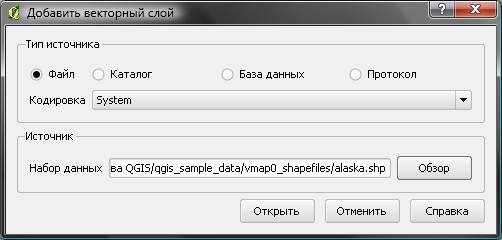
\includegraphics[clip=true, width=12cm]{addvectorlayerdialog}
   \caption{Add Vector Layer Dialog \nixcaption}\label{fig:addvectorlayer}
\end{figure}

\begin{figure}[ht]
   \centering
   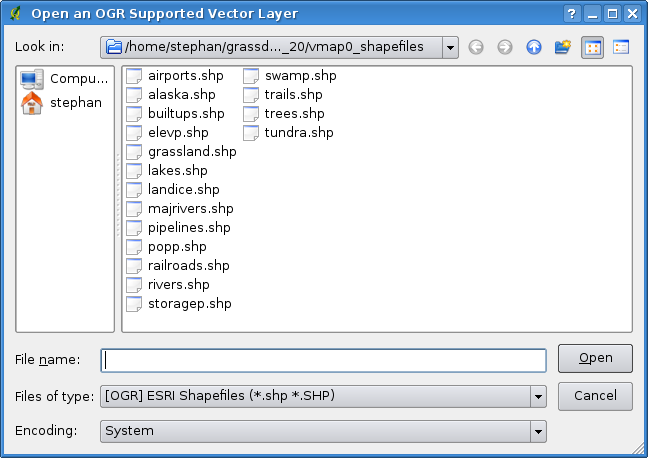
\includegraphics[clip=true, width=12cm]{shapefileopendialog}
   \caption{Open an OGR Supported Vector Layer Dialog \nixcaption}\label{fig:openshapefile}
\end{figure}

\begin{figure}[ht]
   \centering
   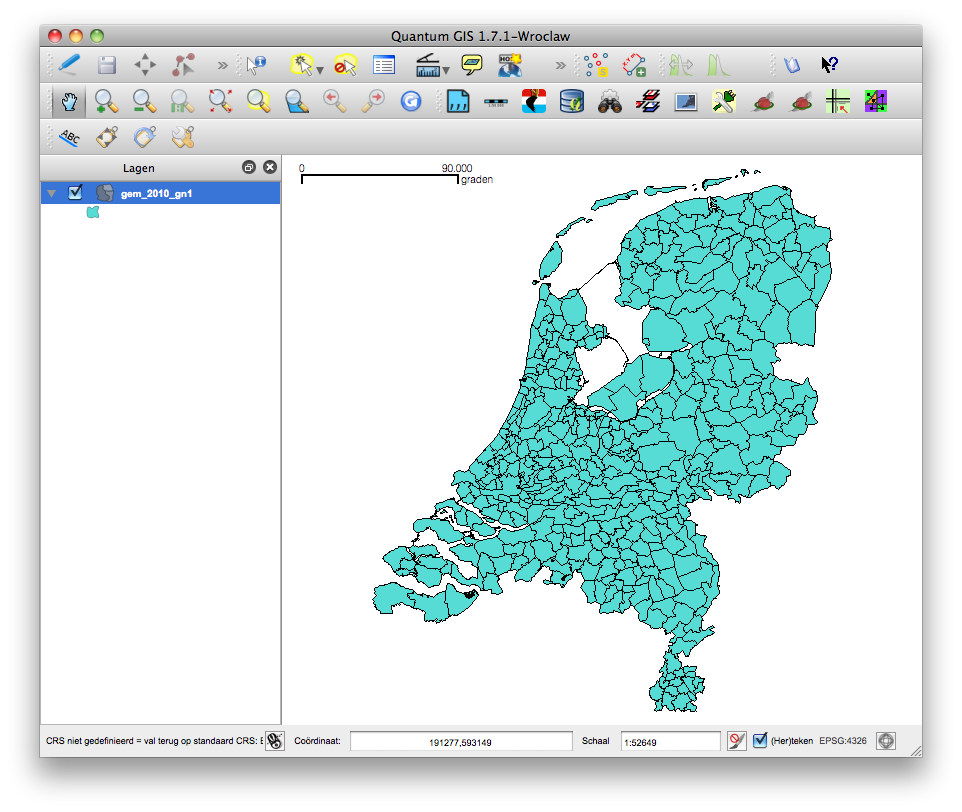
\includegraphics[clip=true, width=12cm]{shapefileloaded}
   \caption{\qg with Shapefile of Alaska loaded \nixcaption}\label{fig:loadedshapefile}
\end{figure}


\includegraphics[width=0.7cm]{mActionAddNonDbLayer} To load a shapefile, start
\qg and click on the \toolbtntwo{mActionAddNonDbLayer}{Add Vector Layer}
toolbar button\index{shapefile!loading} or simply type \keystroke{Ctrl-Shift-V}.
This will bring up a new window (see Figure \ref{fig:addvectorlayer}).

From the available options check \radiobuttonon{File}. Click on \button{Browse}.
That will bring up a standard open file dialog (see Figure
\ref{fig:openshapefile}) which allows you to navigate the file system and load
a shapefile or other supported data source.
The selection box \selectstring{Files of type}{\ldots} allows you to preselect some OGR supported file formats.

You can also select the Encoding type for the shapefile if desired.

Selecting a shapefile from the list and clicking \button{Open} loads it into \qg. Figure
\ref{fig:loadedshapefile} shows \qg after loading the \filename{alaska.shp} file.


\begin{Tip}\caption{\textsc{Layer Colors}}
When you add a layer to the map, it is assigned a random color. When
adding more than one layer at a time, different colors are assigned to each layer.
\end{Tip}

Once loaded, you can zoom around the shapefile using the map navigation tools.
To change the symbology of a layer, open the \dialog{Layer Properties} dialog by double
clicking on the layer name or by right-clicking on the name in the legend and
choosing \dropmenuopt{Properties} from the popup menu. See
Section \ref{sec:symbology} for more information on setting symbology of
vector layers.

\begin{Tip}\caption{\textsc{Load layer and project from mounted external
drives on OS X}}
On OS X, portable drives that are mounted besides the primary hard
drive do not show up under File \arrow Open Project as expected. We are working
on a more OSX-native open/save dialog to fix this. As a workaround you can
type '/Volumes' in the File name box and press return. Then you can navigate
to external drives and network mounts.
\end{Tip}

\subsection{Improving Performance}

To improve the performance of drawing a shapefile, you can create a spatial
index. A \index{spatial index!shapefiles} spatial index will improve the
speed of both zooming and panning. Spatial indexes used by \qg have a
\filename{.qix} extension.

Use these steps to create the index:

\begin{itemize}[label=--]
\item Load a shapefile.
\item Open the \dialog{Layer Properties} dialog by double-clicking on the
shapefile name in the legend or by right-clicking and choosing
\dropmenuopt{Properties} from the popup menu.
\item In the tab \tab{General} click the \button{Create Spatial Index} button.
\end{itemize}

\subsection{Loading a MapInfo Layer}
\index{vector layers!MapInfo}


\includegraphics[width=0.7cm]{mActionAddNonDbLayer} To load a MapInfo layer, click on the \toolbtntwo{mActionAddNonDbLayer}{Add
Vector Layer} toolbar bar button or type \keystroke{Ctrl-Shift-V}, change the
file type filter to \selectstring{Files of Type}{[OGR] MapInfo (*.mif
*.tab *.MIF *.TAB)} and select the layer you want to load.

\subsection{Loading an ArcInfo Binary Coverage}
\index{vector layers!ArcInfo Binary Coverage}


\includegraphics[width=0.7cm]{mActionAddNonDbLayer} To load an ArcInfo binary coverage, click on the
\toolbtntwo{mActionAddNonDbLayer}{Add Vector Layer} toolbar button or type
\keystroke{Ctrl-Shift-V} to open the \dialog{Add Vector Layer} dialog. Select
\radiobuttonon{Directory}. Change to \selectstring {Type}{Arc/Info Binary Coverage}.
Navigate to the directory that contains the coverage files and select it.

Similarly, you can load directory based  vector files in the UK National Transfer Format as well as the
raw TIGER Format of the US Census Bureau.

\section{PostGIS Layers}
\index{vector layers!PostGIS|see{PostGIS}}
\index{PostGIS!layers}
\label{label_postgis}

PostGIS layers are stored in a PostgreSQL database. The advantages of PostGIS
are the spatial indexing, filtering and query capabilities it provides. Using PostGIS,
vector functions such as select and identify work more accurately than with
OGR layers in \qg.

To use PostGIS layers you must:\index{PostgreSQL!loading layers}

\begin{itemize}[label=--]
\item Create a stored connection in \qg to the PostgreSQL database (if one is
not already defined).\index{PostgreSQL!connection}
\item Connect to the database.
\item Select the layer to add to the map.
\item Optionally provide a SQL \usertext{where}
clause to define which features
to load from the layer.
\item Load the layer.
\end{itemize}

\subsection{Creating a stored
Connection}\index{PostgreSQL!connection}\label{sec:postgis_stored}


\includegraphics[width=0.7cm]{mActionAddLayer} The first time
you use a PostGIS data source, you must create a connection to the PostgreSQL
database that contains the data. Begin by clicking on the
\toolbtntwo{mActionAddLayer}{Add PostGIS Layer} toolbar button, selecting the
\dropmenuopttwo{mActionAddLayer}{Add PostGIS Layer...} option from the
\mainmenuopt{Layer} menu or typing \keystroke{Ctrl-Shift-D}. You can also
open the \dialog{Add Vector Layer} dialog and select \radiobuttonon{Database}.
The \dialog{Add PostGIS Table(s)} dialog will
be displayed. To access the connection manager\index{PostgreSQL!connection
manager}, click on the \button{New} button to display the \\
\dialog{Create a New PostGIS Connection} dialog. The parameters required for
a connection are shown in table \ref{tab:postgis_connection_parms}.

\begin{table}[ht]\index{PostgreSQL!connection parameters}
\centering
\caption{PostGIS Connection
Parameters}\label{tab:postgis_connection_parms}\medskip
 \begin{tabular}{|l|p{5in}|}
\hline Name & A name for this connection. Can be the same as \textsl{Database}.
\\
\hline Host \index{PostgreSQL!host}
& Name of the database host. This must be a resolvable host name the same as
would be used to open a telnet connection or ping the host. If the database is
on the same computer as \qg, simply enter 'localhost' here. \\
\hline Database \index{PostgreSQL!database} & Name of the database.  \\
\hline Port \index{PostgreSQL!port}& Port number the PostgreSQL database
server listens on. The default port is 5432.\\
\hline SSL mode \index{PostgreSQL!sslmode}& How the SSL connection will be negotiated with the server. These are the options:
\begin {itemize}
\item disable: only try an unencrypted SSL connection;
\item allow: try a non-SSL connection, if that fails, try an SSL connection;
\item prefer (the default): try an SSL connection, if that fails, try a non-SSL connection;
\item require: only try an SSL connection.
\end {itemize}
Note that massive speedups in PostGIS layer rendering can be achieved by disabling SSL in the connection editor. \\
\hline Username \index{PostgreSQL!username}& User name used to login to the
database. \\
\hline Password \index{PostgreSQL!password}& Password used with
\textsl{Username} to connect to the database.\\
\hline
\end{tabular}
\end{table}

Optional you can activate follwing checkboxes:

\begin{itemize}[label=--]
\item \checkbox{Save Username}
\item \checkbox{Save Password}
\item \checkbox{Only look in the geometry\_columns table}
\item \checkbox{Only look in the 'public' schema}
\item \checkbox{Use estimated table metadata}
\end{itemize}

Once all parameters and options are set, you can test the connection by
clicking on the \button{Test Connect} button\index{PostgreSQL!connection!testing}.

\begin{Tip}\caption{\textsc{\qg User Settings and
Security}}\index{settings}\index{security}
Your customized settings for \qg are stored based on the operating
system. \nix, the settings are stored in your home directory in
\filename{.\qg/}. \win, the settings are stored in the registry. Depending on
your computing environment, storing passwords in your \qg settings may be a
security risk.
\end{Tip}

\subsection{Loading a PostGIS Layer}\index{PostgreSQL!loading layers}


\includegraphics[width=0.7cm]{mActionAddLayer} Once you have one or more
connections defined, you can load layers from the PostgreSQL database. Of
course this requires having data in PostgreSQL. See Section
\ref{sec:loading_postgis_data} for a discussion on importing data into the
database.

To load a layer from PostGIS, perform the following steps:

\begin{itemize}[label=--]
\item If the \dialog{Add PostGIS Table(s)} dialog is not already open, click on the
\toolbtntwo{mActionAddLayer}{Add PostGIS Layer} toolbar button.
\item Choose the connection from the drop-down list and click \button{Connect}.
\item Find the layer you wish to add in the list of available layers.
\item Select it by clicking on it. You can select multiple layers by holding
down the \keystroke{shift} key while clicking. See Section \ref{sec:query_builder} for
information on using the PostgreSQL Query Builder to further define the layer.
\item Click on the \button{Add} button to add the layer to the map.
\end{itemize}

\begin{Tip}\caption{\textsc{PostGIS Layers}}
Normally a PostGIS layer is defined by an entry in the
geometry\_columns table. From version \OLD % should be 0.9.0
on, \qg can load layers that do not have
an entry in the geometry\_columns table. This includes both tables and views.
Defining a spatial view provides a powerful means to visualize your data. Refer
to your PostgreSQL manual for information on creating views.
\end{Tip}

\subsection{Some details about PostgreSQL
layers}\label{sec:postgis_details}
\index{PostgreSQL!layer details}

This section contains some details on how \qg accesses PostgreSQL
layers. Most of the time \qg should simply provide you with a list of
database tables that can be loaded, and load them on request. However,
if you have trouble loading a PostgreSQL table into \qg, the information
below may help you understand any \qg messages and give you direction on
changing the PostgreSQL table or view definition to allow \qg to load it.

\qg requires that PostgreSQL layers contain a column that can be
used as a unique key for the layer. For tables this usually means
that the table needs a primary key, or a column with a unique
constraint on it. In \qg, this column needs to be of
type int4 (an integer of size 4 bytes). Alternatively the ctid column can be
used as primary key. If a table lacks these items,
the oid column will be used instead. Performance will be improved if the
column is indexed (note that primary keys are automatically indexed in
PostgreSQL).

If the PostgreSQL layer is a view, the same requirement exists, but
views don't have primary keys or columns with unique constraints on
them. In this case \qg will try to find a column in the view that is
derived from a suitable table column. It does this by parsing the view
definition SQL. However there are several aspects of SQL that \qg ignores
- these include the use of table aliases and columns that are generated by
SQL functions.

If a suitable column cannot be found, \qg will not load the layer. If this
occurs, the solution is to alter the view so that it does include a suitable
column (a type of int4 and either a primary key or with a unique constraint,
preferably indexed).

%%FIXME: Add missing information
%% When dealing with views, \qg parses the view definition and

\subsection{Importing Data into PostgreSQL}\label{sec:loading_postgis_data}
\index{PostGIS!SPIT!importing data}

\minisec{shp2pgsql}
Data can be imported into PostgreSQL using a number of methods. PostGIS
includes a utility called \filename{shp2pgsql} that can be used to import shapefiles into
a PostGIS enabled database. For example, to import a shapefile named
\filename{lakes.shp}
into a PostgreSQL database named \usertext{gis\_data}, use the following command:

\begin{verbatim}
  shp2pgsql -s 2964 lakes.shp lakes_new | psql gis_data
\end{verbatim}

This creates a new layer named \usertext{lakes\_new} in the
\usertext{gis\_data} database. The
new layer will have a spatial reference identifier (SRID) of 2964. See Section
\ref{label_projections} for more information on spatial reference systems and
projections.
\begin{Tip}
\caption{\textsc{Exporting datasets from PostGIS}\index{PostGIS!Exporting}}
Like the import-tool \filename{shp2pgsql} there is also a tool to export
PostGIS-datasets as shapefiles: \filename{pgsql2shp}. This is shipped within your
PostGIS distribution.
\end{Tip}

\minisec{SPIT Plugin}

\includegraphics[width=0.7cm]{spiticon} \qg comes with a
plugin named
SPIT (Shapefile to PostGIS Import Tool)\index{PostGIS!SPIT}.
SPIT can be used to load multiple shapefiles at one time and includes support
for schemas. To use SPIT, open the Plugin Manager from the \mainmenuopt{Plugins}
menu, check the box next to the \checkbox{SPIT plugin} and click \button{OK}. The SPIT
icon will be added to the plugin toolbar\index{PostGIS!SPIT!loading}.

To import a shapefile, click on the \toolbtntwo{spiticon}{SPIT} tool in the
toolbar to open the \\
\dialog{SPIT - Shapefile to PostGIS Import Tool} dialog. Select the PostGIS database
you want to connect to and click on \button{Connect}. Now you can add one or more
files to the queue by clicking on the \button{Add} button. To process the files,
click on the \button{OK} button. The progress of the import as well as any
errors/warnings will be displayed as each shapefile is processed.

\begin{Tip}\caption{\textsc{Importing Shapefiles Containing
PostgreSQL Reserved Words}}\index{PostGIS!SPIT!reserved words}
If a shapefile is added to the queue containing fields that are
reserved words in the PostgreSQL database a dialog will popup showing the
status
of each field. You can edit the field names\index{PostGIS!SPIT!editing field names}
prior to import and change any that are reserved words (or change any other
field names as desired). Attempting to
import a shapefile with reserved words as field names will likely fail.
\end{Tip}

\minisec{ogr2ogr}
Beside \filename{shp2pgsql} and \filename{SPIT} there is another tool for feeding
geodata in PostGIS: \filename{ogr2ogr}. This is part of your GDAL installation.
To import a shapefile into PostGIS, do the following:
\begin{verbatim}
  ogr2ogr -f "PostgreSQL" PG:"dbname=postgis host=myhost.de user=postgres \
  password=topsecret" alaska.shp
\end{verbatim}

This will import the shapefile \filename{alaska.shp} into the PostGIS-database
\usertext{postgis}
using the user \usertext{postgres} with the password \usertext{topsecret} on host
\server{myhost.de}.

Note that OGR must be built with PostgreSQL to support PostGIS.
You can see this by typing
\begin{verbatim}
ogrinfo --formats | grep -i post
\end{verbatim}

If you like to use PostgreSQL's \filename{COPY}-command instead of the default
\filename{INSERT INTO} method you can export the following
environment-variable (at least available on \nix and \osx):
\begin{verbatim}
  export PG_USE_COPY=YES
\end{verbatim}

\filename{ogr2ogr} does not create spatial indexes like \filename{shp2pgsl}
does. You need to create them manually using the normal SQL-command
\filename{CREATE INDEX} afterwards as an extra step (as described in the next
section \ref{label_improve}).

\subsection{Improving Performance} \label{label_improve}

Retrieving features from a PostgreSQL database can be time consuming,
especially over a network. You can improve the drawing performance of
PostgreSQL layers by ensuring that a \index{PostGIS!spatial index} spatial
index
exists on each layer in the database. PostGIS supports creation of a
\index{PostGIS!spatial index!GiST} GiST
(Generalized Search Tree) index to speed up spatial searches of the data.

The syntax for creating a GiST\footnote{GiST index information is taken from the PostGIS
documentation available at \url{http://postgis.refractions.net}}
index is:

\begin{verbatim}
    CREATE INDEX [indexname] ON [tablename]
      USING GIST ( [geometryfield] GIST_GEOMETRY_OPS );
\end{verbatim}

Note that for large tables, creating the index can take a long time. Once the
index is created, you should perform a \usertext{VACUUM ANALYZE}. See the
PostGIS documentation \cite{PostGISweb} for more information.

The following is an example of creating a GiST index:
\begin{verbatim}
gsherman@madison:~/current$ psql gis_data
Welcome to psql 8.3.0, the PostgreSQL interactive terminal.

Type:  \copyright for distribution terms
        \h for help with SQL commands
        \? for help with psql commands
        \g or terminate with semicolon to execute query
        \q to quit

gis_data=# CREATE INDEX sidx_alaska_lakes ON alaska_lakes
gis_data-# USING GIST (the_geom GIST_GEOMETRY_OPS);
CREATE INDEX
gis_data=# VACUUM ANALYZE alaska_lakes;
VACUUM
gis_data=# \q
gsherman@madison:~/current$
\end{verbatim}

\subsection{Vector layers crossing 180$^\circ$ longitude}
\index{vector layers!crossing}

Many GIS packages don't wrap vector maps, with a geographic reference system
(lat/lon), crossing the \degrees{180} longitude line. As result, if
we open such map in \qg, we will see two far, distinct locations, that
should show near each other. In Figure \ref{fig:vector_not_wrapping} the tiny
point on the far left of the map canvas (Chatham Islands), should be within
the grid, right of New Zealand main islands.

\begin{figure}[ht]
   \centering
   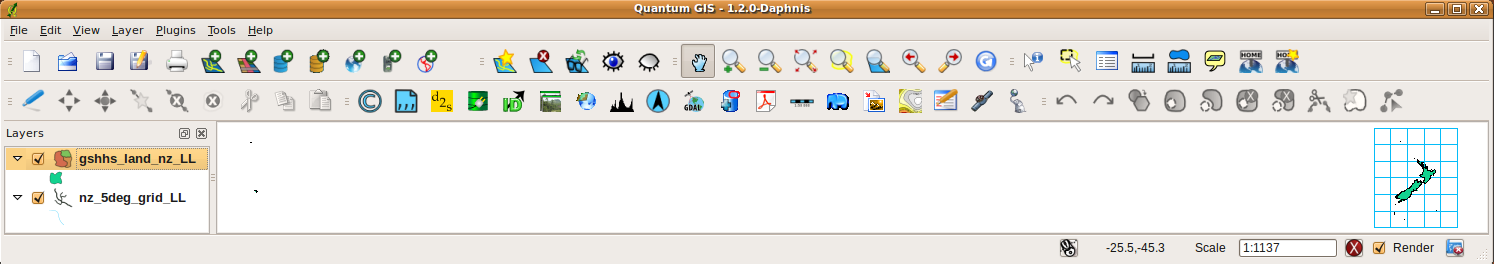
\includegraphics[clip=true, width=\textwidth]{vectorNotWrapping}
      \caption{Map in lat/lon crossing the \degrees{180} longitude line \nixcaption}
   \label{fig:vector_not_wrapping}
\end{figure}

A workaround is to transform the longitude values using PostGIS and the
\textbf{ST\textunderscore Shift\textunderscore Longitude}
\footnote{\url{http://postgis.refractions.net/documentation/manual-1.4/ST\_Shift\_Longitude.html}}
function. This function reads every point/vertex in every component of every
feature in a geometry, and if the longitude coordinate is < \degrees{0} adds
\degrees{360} to it. The result would be a \degrees{0} - \degrees{360} version of
the data to be plotted in a \degrees{180} centric map.

\begin{figure}[ht]
   \centering
   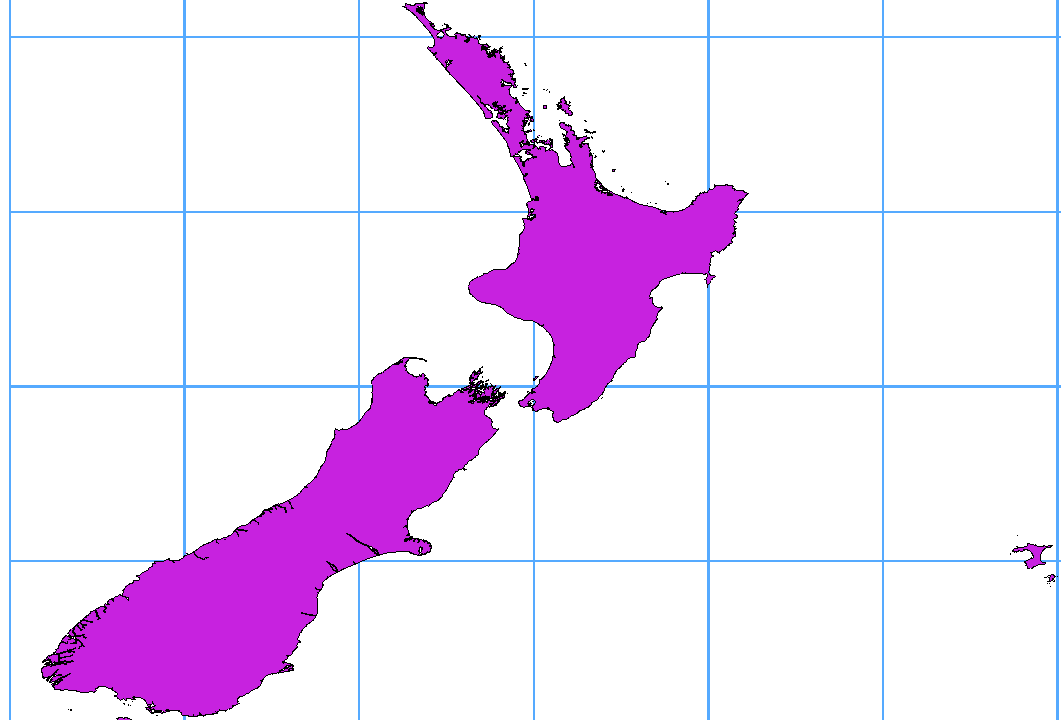
\includegraphics[clip=true, width=9cm]{vectorWrapping}
   \caption{Map crossing \degrees{180} longitude applying the ST\textunderscore Shift\textunderscore Longitude function \nixcaption}
\label{fig:vector_wrapping}
\end{figure}

\minisec{Usage}

\begin{itemize}[label=--]
\item Import data to PostGIS (\ref{sec:loading_postgis_data}) using for
example the PostGIS Manager plugin or the SPIT plugin
\item Use the PostGIS command line interface to issue the following command
(this is an example where "TABLE" is the actual name of your PostGIS table) \\
\texttt{gis\_data=\# update TABLE set the\_geom=ST\_shift\_longitude(the\_geom);}
\item If everything went right you should receive a confirmation about the
number of features that were updated, then you'll be able to load the map and
see the difference (Figure \ref{fig:vector_wrapping})
\end{itemize}

\section{SpatiaLite Layers}
\index{SpatiaLite layers!properties dialog}
\index{vector layers!SpatlaLIte|see{SpatiaLite}}
\index{SpatiaLite!layers}
\label{label_spatialite}


\includegraphics[width=0.7cm]{mActionAddSpatiaLiteLayer}
The first time you load data from a SpatiaLite database, begin by clicking on the
\toolbtntwo{mActionAddSpatiaLiteLayer}{Add SpatiaLite Layer} toolbar button or by selecting the
\dropmenuopttwo{mActionAddSpatiaLiteLayer}{Add SpatiaLite Layer...}
option from the \mainmenuopt{Layer} menu or by typing \keystroke{L}.
This will bring up a window, which will allow you to either connect to a SpatiaLite 
database already known to \qg, which you can choose from the dropdown menu or to define 
a new connection to a new database. To define a new connection, click on \button{New} and 
use the file browser to point to your SpatiaLite database, which is a file with 
a \filename{.sqlite } extension.

If you want to save a vector layer to SpatiaLite format you can do this opening the right 
mouse menu of the layer. Then click on \dropmenuopt{Save as}, define the name of the output 
file, sqlite as format and the CRS and then add 'SPATIALITE=YES' in the OGR data source 
creation option field. This tells OGR to create a SpatiaLite database. See 
also \url{http://www.gdal.org/ogr/drv_sqlite.html}.

\section{The Vector Properties Dialog}\label{sec:vectorprops}
\index{vector layers!properties dialog}

The \dialog{Layer Properties} dialog for a vector layer provides information
about the layer, symbology settings and labeling options. If your vector
layer has been loaded from a PostgreSQL/PostGIS datastore, you can also alter
the underlying SQL for the layer by invoking the \dialog{Query Builder}
dialog on the \tab{General} tab.
To access the \dialog{Layer Properties} dialog, double-click on a layer in
the legend or right-click on the layer and select \dropmenuopt{Properties}
from the popup menu.

\begin{figure}[ht]
   \centering
   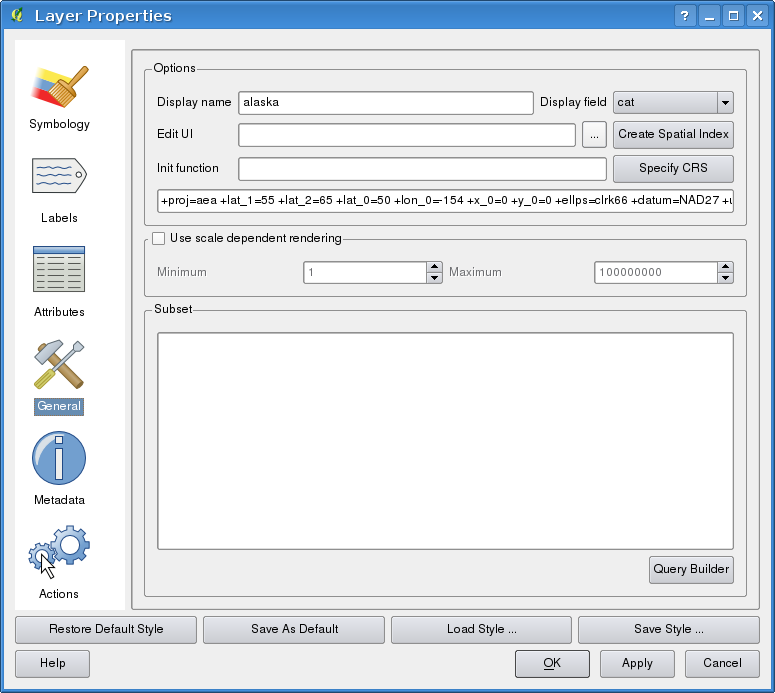
\includegraphics[clip=true, width=12cm]{vectorLayerSymbology}
   \caption{Vector Layer Properties Dialog \nixcaption}\label{fig:vector_symbology}
 \end{figure}

\subsection{Symbology Tab}\label{sec:symbology}
\index{vector layers!symbology}

\qg supports a number of symbology renderers to control how
vector features are displayed. Currently the following renderers
are available:

\begin{description}
    \item[Single symbol] - a single style is applied to every
    object in the layer.\index{vector layers!renderers!single symbol}
    \item[Graduated symbol] - objects within the layer are
    displayed with different symbols classified by the values of a
    particular field.\index{vector layers!renderers!graduated symbol}
    \item[Continuous color] - objects within the layer are
    displayed with a spread of colours classified by the numerical
    values within a specified field.\index{vector layers!renderers!continuous
color}
    \item[Unique value] - objects are classified by the unique
    values within a specified field with each value having a
    different symbol.\index{vector layers!renderers!unique value}
\end{description}

To change the symbology for a layer, simply double click on its legend
entry and the vector \dialog{Layer Properties} dialog will be
shown.\index{symbology!changing}

\begin{figure}[ht]
\centering
\caption{Symbolizing Options \nixcaption}
   \subfloat[Single symbol] {\label{subfig:single_symbol}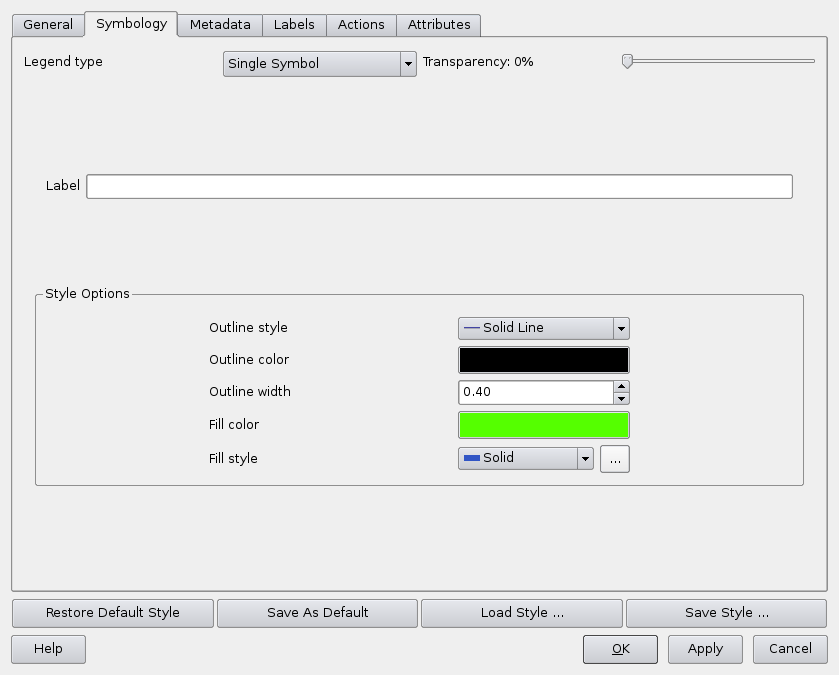
\includegraphics[clip=true, width=0.4\textwidth]{vectorClassifySingle}}
   \hspace{1cm}
   \subfloat[Graduated symbol] {\label{subfig:graduated_symbol}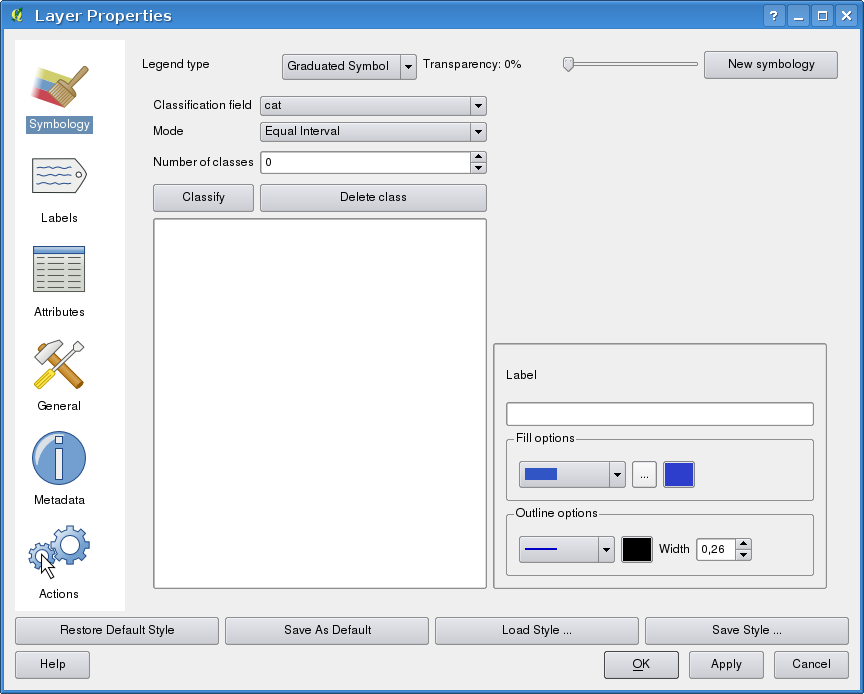
\includegraphics[clip=true, width=0.4\textwidth]{vectorClassifyGraduated}}
   \hspace{1cm}
   \subfloat[Continous color] {\label{subfig:cont_color}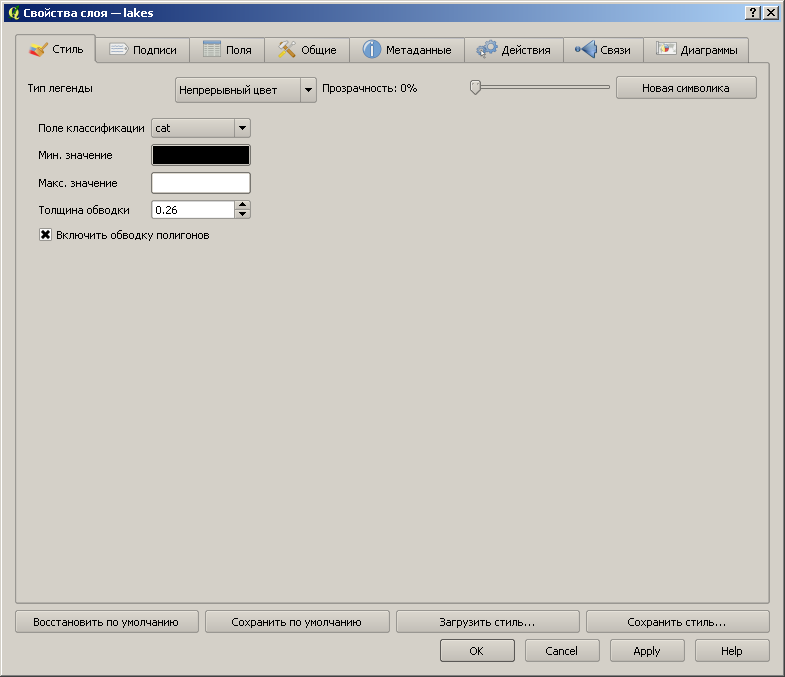
\includegraphics[clip=true, width=0.4\textwidth]{vectorClassifyContinous}}
   \hspace{1cm}
   \subfloat[Unique value] {\label{subfig:unique_val}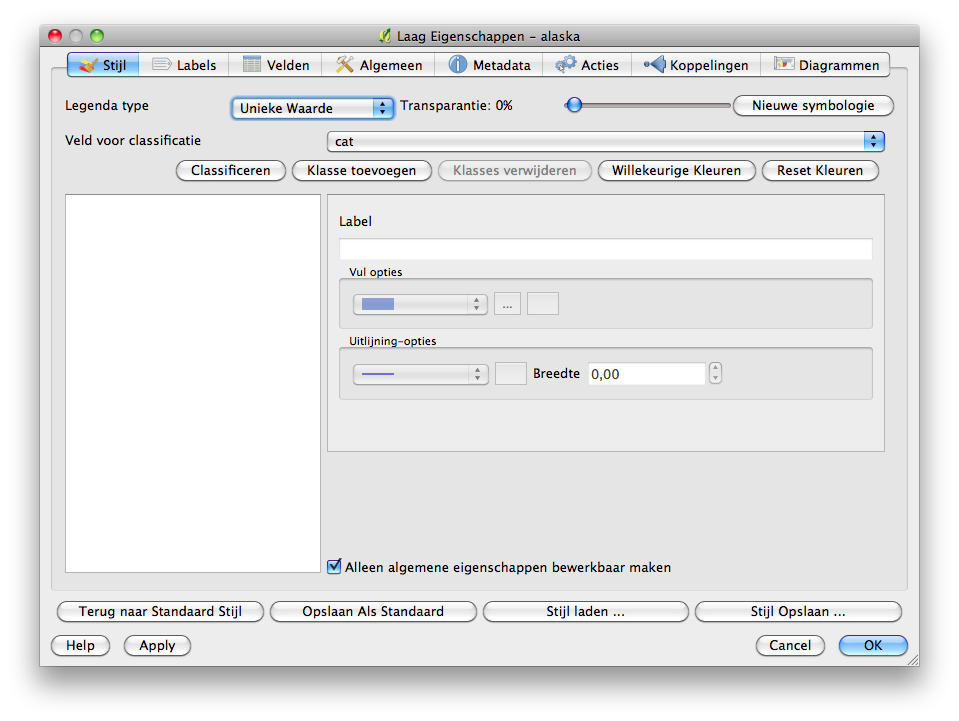
\includegraphics[clip=true, width=0.4\textwidth]{vectorClassifyUnique}}
\end{figure}

% FIXME: outdated
% Since \usertext{version v0.9} there is a function to use image files stored on
% your computer as fill pattern for vector layers.

\minisec{Style Options} \label{sec:style_options} \index{vector layers!styles}
Within this dialog you can style your vector layer. Depending on the selected
rendering option you have the possibility to also classify your mapfeatures.

At least the following styling options apply for nearly all renderers:
\begin{description}
\item[Fill options]
\begin{description}
 \item[Fill style] - Style for filling. Beside the given brushes you can
 select \selectstring{Fill style}{? Texture} and click the \browsebutton
 button for selecting your own texture file. Currently the fileformats
 \filename{*.jpeg, *.xpm, and *.png} are supported.
 \item[Fill color] - fill-color of your features.
\end{description}
\item[Outline options]
\begin{description}
 \item[Outline style] - pen-style for your outline of your feature. You can
 also set this to 'no pen'.
 \item[Outline color] - color of the ouline of your feature.
 \item[Outline width] - width of your features.
\end{description}
\end{description}

Once you have styled your layer you also could save your layer-style to a
separate file (with \filename{*.qml}-ending).
To do this, use the button \button{Save Style \ldots}. No need to say that
\button{Load Style \ldots} loads your saved layer-style-file.

If you wish to always use a particular style whenever the layer is loaded,
use the \button{Save As Default} button to make your style the default. Also,
if you make changes to the style that you are not happy with, use the \button{Restore
Default Style} button to revert to your default style.

\minisec{Vector transparency} \label{sec:vect_transparency}
\index{vector layers!transparency}

\qg allows to set a transparency for every vector layer. This can be done with
the slider \\
\slider{Transparency} inside the \tab{symbology} tab (see
fig. \ref{subfig:single_symbol}). This is very useful for overlaying several
vector layers.

\subsection{New Generation Symbology}

Since \qg 1.4.0  a new symbology was integrated in parallel with the symbology
described above. This new generation symbology provides a variety of improvements and
new features and will replace the current symbology in one of the upcoming releases.
To switch to the new symbolgy you currently have to click on the \button{New symbology} button in the \tab{General} tab of the \dialog{Layer Properties} dialog. You can
also make the New symobolgy the default, activating \checkbox{Use new generation symbology for rendering} in the \tab{Rendering \& SVG} tab under the \mainmenuopt{Settings} \arrow \dropmenuopt{Options} menu.

\minisec{Understanding the new generation symbology}

There are three types of symbols: marker symbols (for points), line symbols and
fill symbols (for polygons). Symbols can consist of one or more symbol layers. It
is possible to define the color of a symbol and this color is then defined for all
symbol layers. Some layers may have the color locked - for those the color can not
be altered. This is useful when you define the color of a multilayer symbol.
Similarly, it is possible to define the width for line symbols, as well as size and
angle for marker symbols.

\minisec{Available symbol layer types}

\begin{itemize}[label=--]
\item \textbf{Simple marker}: Rendering with one of hardcoded markers.
\item \textbf{Simple line}: Usual rendering of a line (with specified
width, color and pen style).
\item \textbf{Simple fill}: Usual rendering of a polygon (with defined
fill color, fill pattern and outline).
\item \textbf{SVG marker}: Rendering with a SVG picture.
\item \textbf{Marker line}: A line rendered by repeating a marker symbol.
\end{itemize}

\minisec{Color ramps}

Color ramps are used to define a range of colors that can be used during
the creation of renderers. The symbol's color will be set from the color ramp.

There are three types of color ramps:

\begin{itemize}[label=--]
\item \textbf{Gradient}: Linear gradient from one color to some other.
\item \textbf{Random}: Randomly generated colors from a specified area of
color space.
\item \textbf{ColorBrewer}: Create color area from a color shema and a defined
number of color classes.
\end{itemize}

Color ramps can be defined in the \dialog{Style Manager} dialog (see Section
\ref{subsec:stylemanager}) by selecting \\
\selectstring{Style item type:}{Color ramp} as style element type from the drop-down list, clicking on \button{Add item} button and then choosing a color ramp type.

\minisec{Styles}

A style groups a set of various symbols and color ramps. You can define your
prefered or frequently used symbols, and can use it  without having to recreate
it everytime. Style items (symbols and color ramps) have always a name by which
they can be queried from the style. There is one default style in \qg (modifiable)
and the user can add further styles.

\minisec{Renderers}

The renderer is responsible for drawing a feature together with the correct
symbol. There are three types of renderers: single symbol, categorized (called
unique color in the old symbology), and graduated. There is no continuous color
renderer, because it is in fact only a special case of the graduated renderer.
The categorized and graduated renderer can be created by specifying a symbol
and a color ramp - they will set the colors for symbols appropriately.

\subsection{Working with the New Generation Symbology}

First you have to enable the new generation symbology clicking on the
\button{New symbology} button in the \tab{Symbology} tab of the
\dialog{Layer Properties} dialog. The new dialog allows to choose one of the
three renderers: single symbol, categorized and graduated. Depending on the
chosen renderer, the symbology tab provides different settings and options, that
will be described in the following sections. The new generation symbology dialog 
also provides a \button{Style Manager} button which gives access to the Style 
Manager (see section \ref{subsec:stylemanager}). The Style Manager allows you to 
edit and remove existing symbols and add new ones. 

\minisec{Single Symbol Renderer}

The Single Symbol Renderer is used to render all features of the layer using a
single user-defined symbol. The properties, that can be adjusted in the
Symbology tab, depend partially on the type of the layer, but all types share
the following structure. In the top left part of the tab, there is a preview of
the current symbol to be rendered. In the bottom part of the tab, there is a
list of symbols already defined for the current style, prepared to be used via
selecting them from the list. The current symbol can be modified using the
\button{Properties} button, which opens a \dialog{Symbol Properties} dialog, or
the \button{Set Color} button, which opens an ordinary \dialog{Color} dialog.
After having done any needed changes, the symbol can be added to the list of
current style symbols (using the \button{Add to style} button) and then easily
be used in the future.

\textbf{Note}: To modify line width, besides modifying the symbol itself, you
can use data-defined Size Scale (available through \button{Advanced} next to 
\button{Add to Style}).

\begin{figure}[ht]
\centering
   \subfloat[Single symbol point properties] {\label{subfig:singleNG1}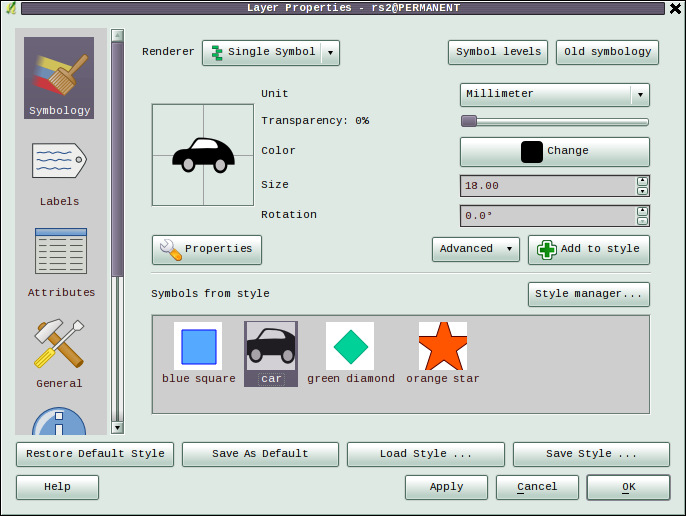
\includegraphics[clip=true, width=0.3\textwidth]{singlesymbol_ng_point}}
   \hspace{1cm}
   \subfloat[Single symbol line properties] {\label{subfig:singleNG2}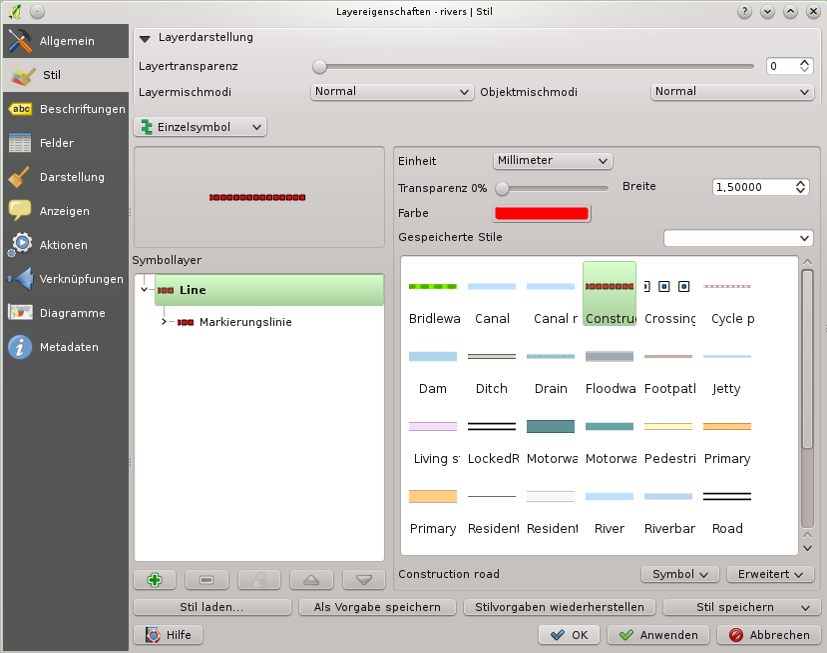
\includegraphics[clip=true, width=0.3\textwidth]{singlesymbol_ng_line}}
   \hspace{1cm}
   \subfloat[Single symbol area properties] {\label{subfig:singleNG3}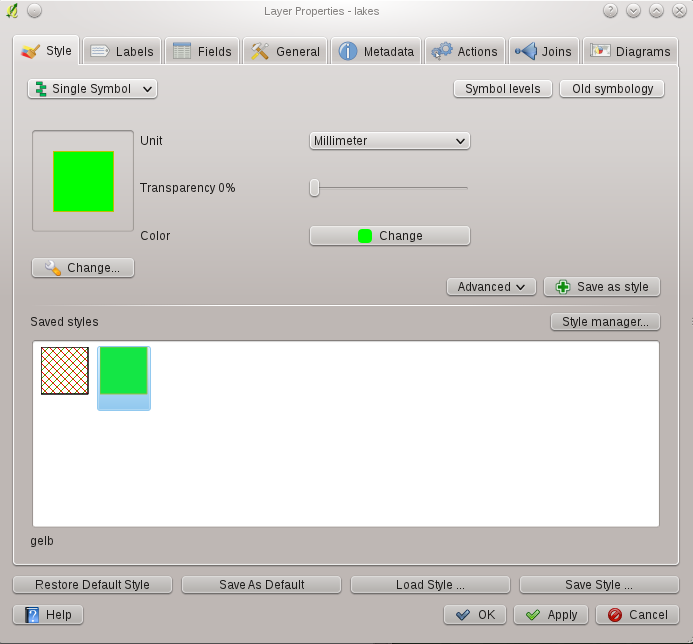
\includegraphics[clip=true, width=0.3\textwidth]{singlesymbol_ng_area}}
\caption{New Single Symbolizing options \nixcaption}
\end{figure}

\minisec{Categorized Renderer}

The Categorized Renderer is used to render all features from a layer, using a
single user-defined symbol, which color reflects the value of a selected
feature's attribute. The Symbology tab allows you to select:

\begin{itemize}[label=--]
\item The attribute (using the Column listbox)
\item The symbol (using the Symbol Properties dialog)
\item The colors (using the Color Ramp listbox)
\end{itemize}

The Advanced button in the lower right corner of the dialog allows to set
th fields containing rotation and size scale information.
For convenience, the list in the bottom part of the tab lists the values of
all currently selected attributes together, including the symbols that will
be rendered.

The example in figure \ref{fig:catsymNG} shows the category rendering dialog
used for the rivers layer of the \qg sample dataset.

\begin{figure}[ht]
   \centering
   \caption{New Categorized Symbolizing options \nixcaption}\label{fig:catsymNG}
   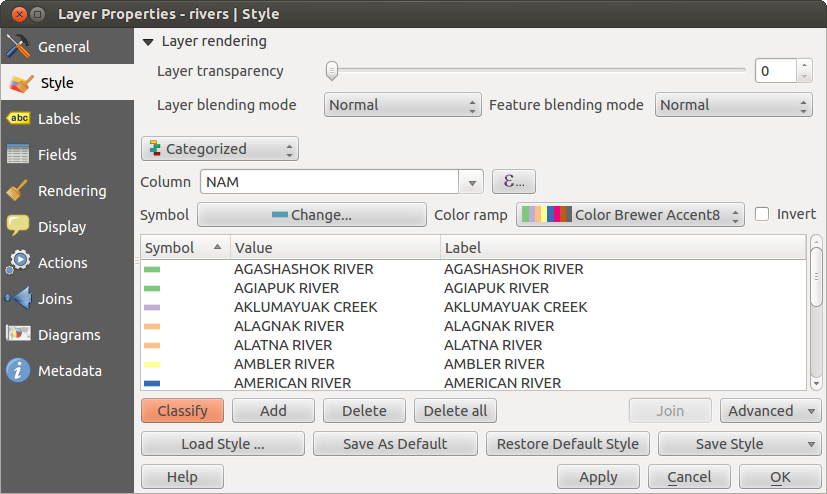
\includegraphics[clip=true, width=10cm]{categorysymbol_ng_line}
\end{figure}

You can create a custom color ramp choosing New color ramp... from the Color 
ramp dropdown menu. A dialog will prompt for the ramp type: Gradient, Random,
ColorBrewer, then each one has options for number of steps and/or multiple
stops in the color ramp. See \ref{fig:ccrg} for an example of custom color
ramp.

\begin{figure}[ht]
   \centering
   \caption{Example of custom gradient color ramp with multiple stops \nixcaption}\label{fig:ccrg}
   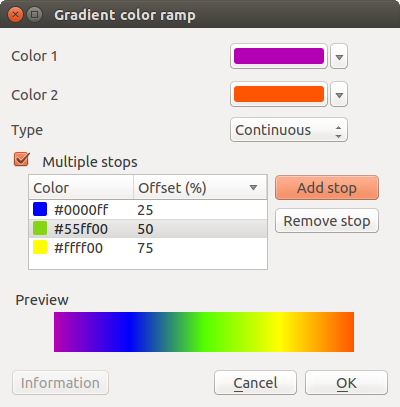
\includegraphics[clip=true, width=10cm]{customColorRampGradient.png}
\end{figure}

\minisec{Graduated Renderer}

The Graduated Renderer is used to render all the features from a layer, using
a single user-defined symbol, whose color reflects the classification of a selected
feature's attribute to a class. Like Categorized Renderer, it allows to define
rotation and size scale from specified columns.

Analogue to the categorized rendered, the symbology tab allows you to select:

\begin{itemize}[label=--]
\item The attribute (using the Column listbox)
\item The symbol (using the Symbol Properties button)
\item The colors (using the Color Ramp list)
\end{itemize}

Additionally, you can specify the number of classes and also the mode how to
classify features inside the classes (using the Mode list). The available modes are:
\begin{itemize}
 \item Equal Interval
 \item Quantile
 \item Natural Breaks (Jenks)
 \item Standard Deviation
 \item Pretty Breaks
\end{itemize}

The listbox in the  bottom part of the symbology tab lists the classes together with their ranges,
labels and symbols that will be rendered.

The example in figure \ref{fig:gradsymNG} shows the graduated rendering dialog
for the rivers layer of the \qg sample dataset.

\begin{figure}[ht]
   \centering
   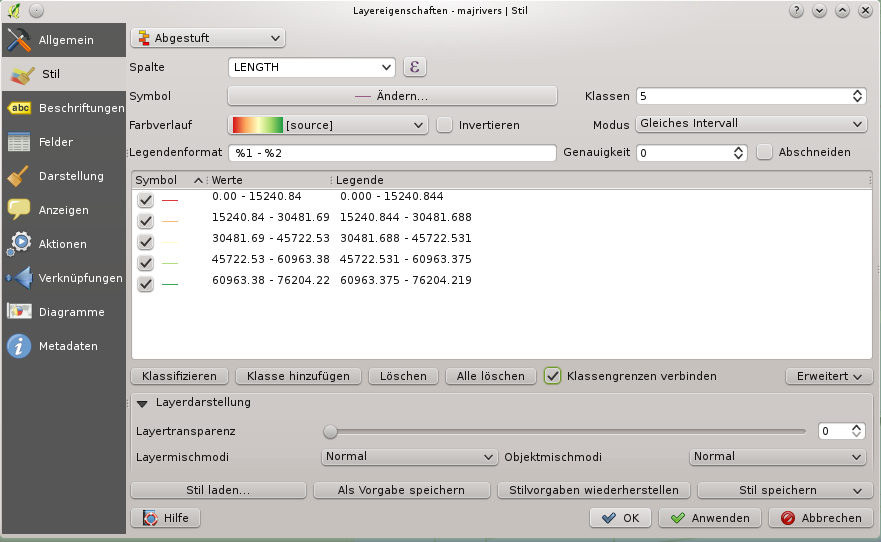
\includegraphics[clip=true, width=10cm]{graduatesymbol_ng_line}
   \caption{New Graduated Symbolizing options \nixcaption}\label{fig:gradsymNG}
\end{figure}

\minisec{Rule-based rendering}

The rule-based renderer is used to render all the features from a layer, using
rule based symbols, whose color reflects the classification of a selected
feature's attribute to a class.

The example in figure \ref{fig:rulesymNG} shows the rule-based rendering dialog
for the rivers layer of the \qg sample dataset.

\begin{figure}[ht]
   \centering
   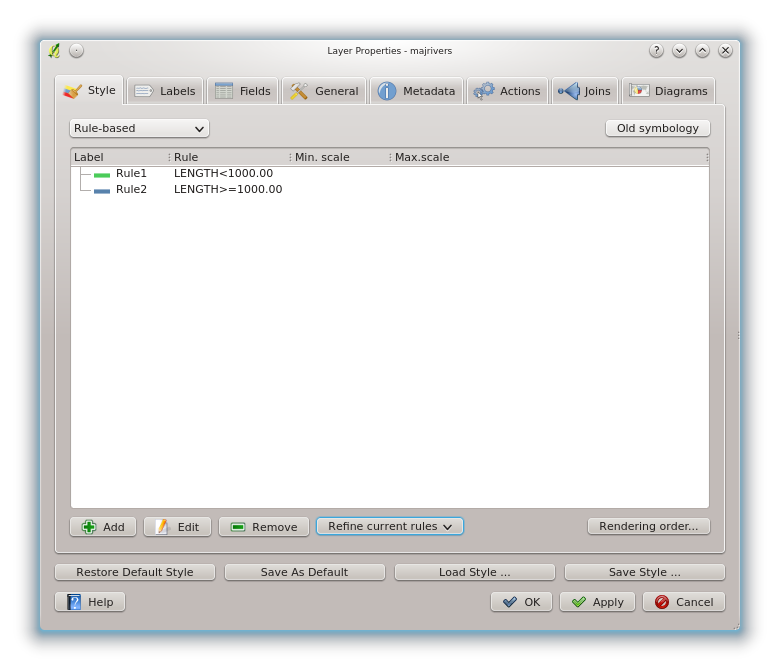
\includegraphics[clip=true, width=10cm]{rulesymbol_ng_line}
   \caption{New Rule-based Symbolizing options \nixcaption}\label{fig:rulesymNG}
\end{figure}

\minisec{Point displacement}

The point displacement renderer offers to visualize all features of a point
layer, even if they have the same location. To do this, the symbols of the
points are placed on a displacement circle around a center symbol.

\begin{figure}[ht]
   \centering
   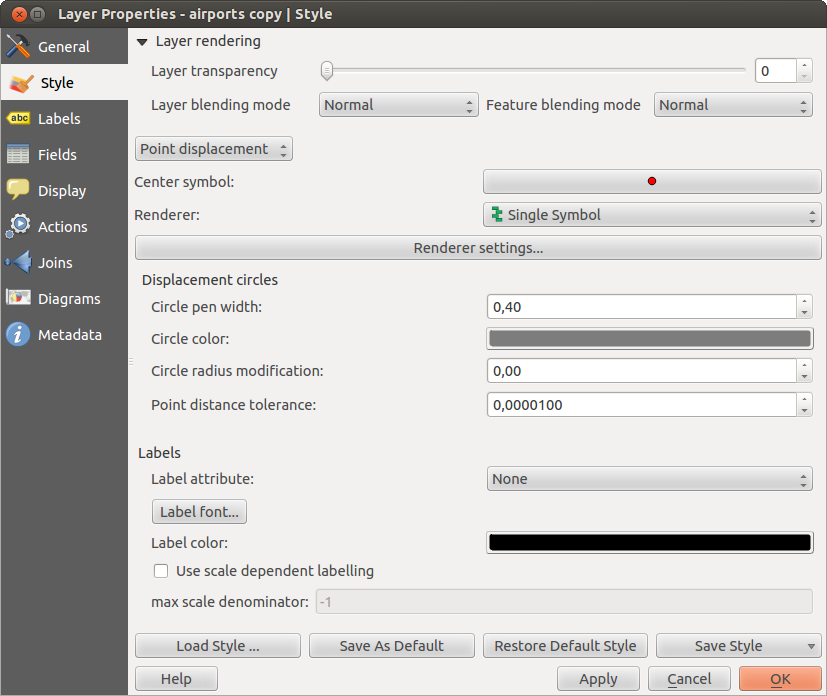
\includegraphics[clip=true, width=10cm]{poi_displacement}
   \caption{Point displacement dialog \nixcaption}\label{fig:poidissymNG}
\end{figure}

\minisec{Symbol Properties}

The symbol properties dialog allows the user to specify different properties of
the symbol to be rendered. In the top left part of the dialog, you find a preview
of the current symbol as it will be displayed in the map canvas. Below the preview
is the list of symbol layers. To start the symbol properties dialog, click the
\dropmenuopttwo{mActionOptions}{Properties} button in the \tab{Symbology} tab of the
\dialog{Layer Properties} dialog.

The control panels allow adding or removing layers, changing the position of layers,
or locking layers for color changes. In the right part of the dialog, there are
shown the settings applicable to the single symbol layer selected in the symbol
layer list. The most important is the 'Symbol Layer Type' combo box, which allows
you to choose the layer type. The available options depend on the layer type
(Point, Line, Polygon).

\begin{description}
\item Symbol layer type options for point layers
\begin{itemize}[label=--]
\item \textbf{SimpleMarker}: Border color, Fill color, Size, Angle, Offset X,Y
\item \textbf{SvgMarker}: Size, Angle, Offset X,Y, SVG Image
\end{itemize}
\item Symbol layer type options for line layers
\begin{itemize}[label=--]
\item \textbf{LineDecoration}: Color
\item \textbf{MarkerLine}: Marker, Marker Interval, Rotate marker, Line offset
\item \textbf{SimpleLine}: Color, Pen width, pen style, Offset, Join style and Cap style
\end{itemize}
\item Symbol layer type options for polygon layers
\begin{itemize}[label=--]
\item \textbf{SimpleFill}: Color, Fill style, Border color, Border style, Border width
\end{itemize}
\end{description}


\begin{figure}[ht]
\centering
   \subfloat[Line composed from three simple lines] {\label{subfig:symprops1}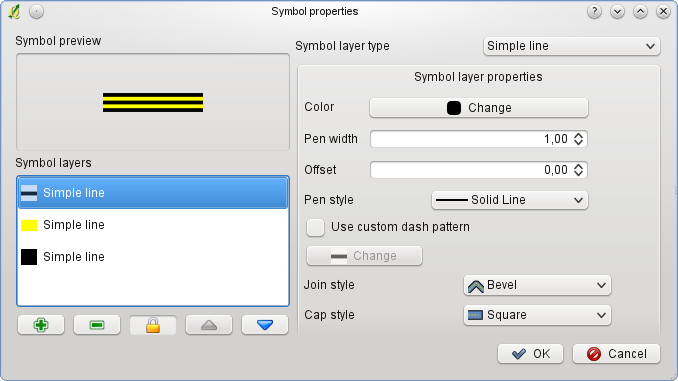
\includegraphics[clip=true, width=0.3\textwidth]{symbolproperties1}}
   \hspace{1cm}
   \subfloat[Symbol properties for point layer] {\label{subfig:symprops2}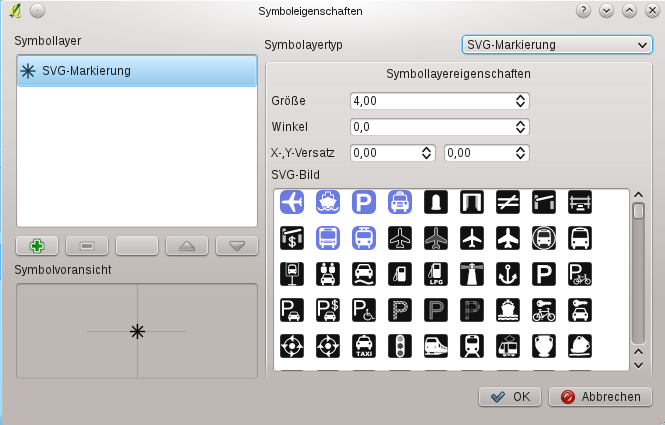
\includegraphics[clip=true, width=0.3\textwidth]{symbolproperties2}}
   \hspace{1cm}
   \subfloat[Filling pattern for a polygon] {\label{subfig:symprops3}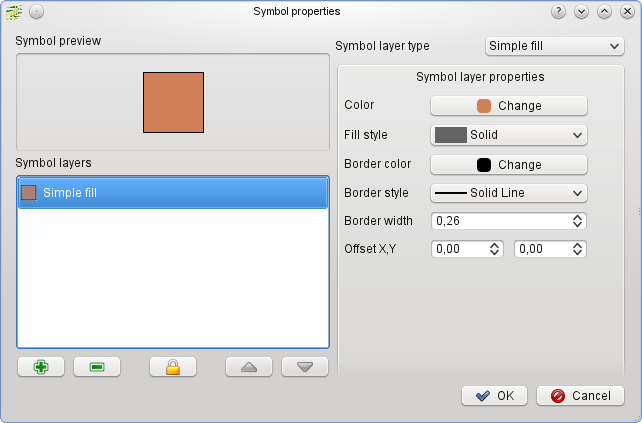
\includegraphics[clip=true, width=0.3\textwidth]{symbolproperties3}}
\caption{Defining symbol properties \nixcaption}
\end{figure}

\subsection{Style Manager to manage symbols and color ramps}\label{subsec:stylemanager}

The Style Manger is a small helper application, that lists symbols and color
ramps available in a style. It also allows you to add and/or remove items. To
launch the Style Manager, click on \mainmenuopt{Settings} \arrow \dropmenuopt{Style
Manager} in the main menu.

\begin{figure}[ht]
   \centering
   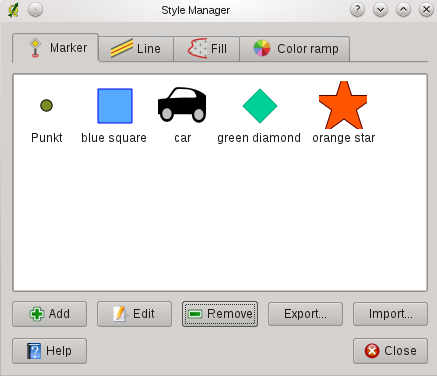
\includegraphics[clip=true, width=7cm]{stylemanager}
   \caption{Style Manager to manage symbols and color ramps \nixcaption}\label{fig:stylemanager}
\end{figure}

\subsection{Labels Tab}\label{labeltab}

The \tab{Labels} tab allows you to enable labeling features and control a number of
options related to fonts, placement, style, alignment and buffering.

We will illustrate this by labelling the lakes shapefile of the
\filename{\qg\_example\_dataset}:

\begin{enumerate}
\item Load the Shapefile \filename{alaska.shp} and GML file \filename{lakes.gml} in \qg.
\item Zoom in a bit to your favorite area with some lake.
\item Make the \filename{lakes} layer active.
\item Open the \dialog{Layer Properties} dialog.
\item Click on the \tab{Labels} tab.
\item Check the \checkbox{Display labels} checkbox to enable labeling.
\item Choose the field to label with.
  We'll use \selectstring{Field containing label}{NAMES}.
\item Enter a default for lakes that have no name. The default label will be
  used each time \qg encounters a lake with no value in the \guilabel{NAMES}
field.
\item If have labels extending over several lines, check \checkbox{Multiline
labels?}. \qg will check for a true line return in your label field and
insert the line breaks accordingly. A true line return is a \textbf{single}
character \textbackslash n, (not two separate characters, like a backlash
\textbackslash ~followed by the character n).
\item Click \button{Apply}.
\end{enumerate}

Now we have labels. How do they look? They are probably too big and poorly
placed in relation to the marker symbol for the lakes.

Select the \tab{Font} entry and use the \button{Font} and \button{Color}
buttons to set the font and color. You can also change the angle and the
placement of the text-label.

To change the position of the text relative to the feature:

\begin{enumerate}
\item Click on the \tab{Font} entry.
\item Change the placement by selecting one of the radio buttons
in the \classname{Placement} group. To fix our labels, choose the
\radiobuttonon{Right} radio button.
\item the \classname{Font size units} allows you to select between
\radiobuttonon{Points} or \radiobuttonon{Map units}.
\item Click \button{Apply} to see your changes without closing the dialog.
\end{enumerate}

Things are looking better, but the labels are still too close to the marker. To
fix this we can use the options on the \tab{Position} entry. Here we can add
offsets for the X and Y directions. Adding an X offset of 5 will move our
labels off the marker and make them more readable. Of course if your marker
symbol or font is larger, more of an offset will be required.

The last adjustment we'll make is to \tab{Buffer} the labels. This just means
putting a backdrop around them to make them stand out better. To buffer the
lakes labels:

\begin{enumerate}
\item Click the \tab{Buffer} tab.
\item Click the \checkbox{Buffer Labels?} checkbox to enable buffering.
\item Choose a size for the buffer using the spin box.
\item Choose a color by clicking on \button{Color} and choosing your
  favorite from the color selector. You can also set some transparency for the
  buffer if you prefer.
\item Click \button{Apply} to see if you like the changes.
\end{enumerate}

If you aren't happy with the results, tweak the settings and then test again
by clicking \button{Apply}.

A buffer of 1 points seems to give a good result.
Notice you can also specify the buffer size in map units if that works out
better for you.

The remaining entries inside the \tab{Label} tab allow you control the appearance of the
labels using attributes stored in the layer. The entries beginning with \tab{Data defined} allow you to
set all the parameters for the labels using fields in the layer.

Not that the \tab{Label} tab provides a \classname{preview-box} where your
selected label is shown.

\subsection{New Labeling}\index{New labeling}\label{newlabel}

The new \toolbtntwo{labeling}{Labeling} core application provides smart labeling
for vector point,  line and polygon layers and only requires a few parameters.
This new application will replace the current QGIS labeling, described in section
\ref{labeltab} and also supports on-the-fly transformated layers.

\minisec{Using new labeling}

\begin{enumerate}
  \item Start QGIS and load a vector point, line or polygon layer.
  \item Activate the layer in the legend and click on the
  \toolbtntwo{labeling}{Labeling} icon in the QGIS toolbar menu.
\end{enumerate}

\minisec{Labeling point layers}

First step is to activate the \checkbox{Label this layer} checkbox and select an attribute
column to use for labeling. After that you can define the label placement and text style,
labeling priority, scale-based visibility, if every part of multipart feature is to be
labeled and if features act as obstacles for labels or not (see
Figure \ref{fig:pointlabel}).

\begin{figure}[ht]
\centering
   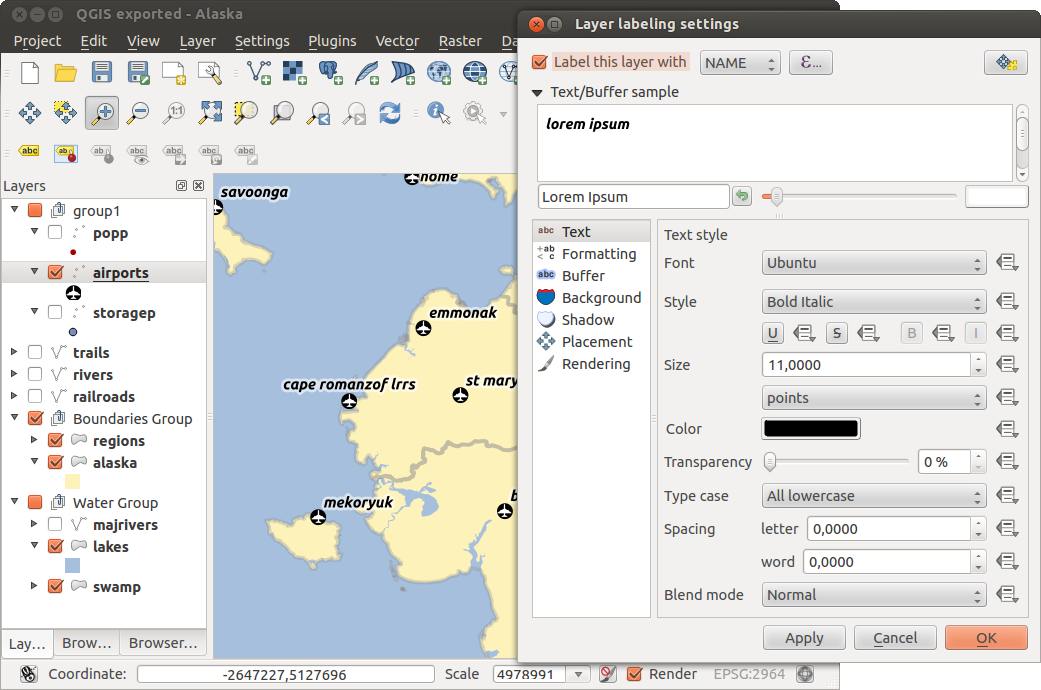
\includegraphics[clip=true, width=10cm]{label_points}
   \caption{Smart labeling of vector point layers \nixcaption}\label{fig:pointlabel}
\end{figure}

\minisec{Labeling line layers}

First step is to activate the \checkbox{Label this layer} checkbox and select an attribute
column to use for labeling. After that you can define the label placement, orientation,
distance to feature, text style, labeling priority, scale-based visibility, if every part
of a multipart line is to be labeled, if lines shall be merged to avoid duplicate labels
and if features act as obstacles for labels or not (see Figure \ref{fig:linelabel}).

\begin{figure}[ht]
\centering
   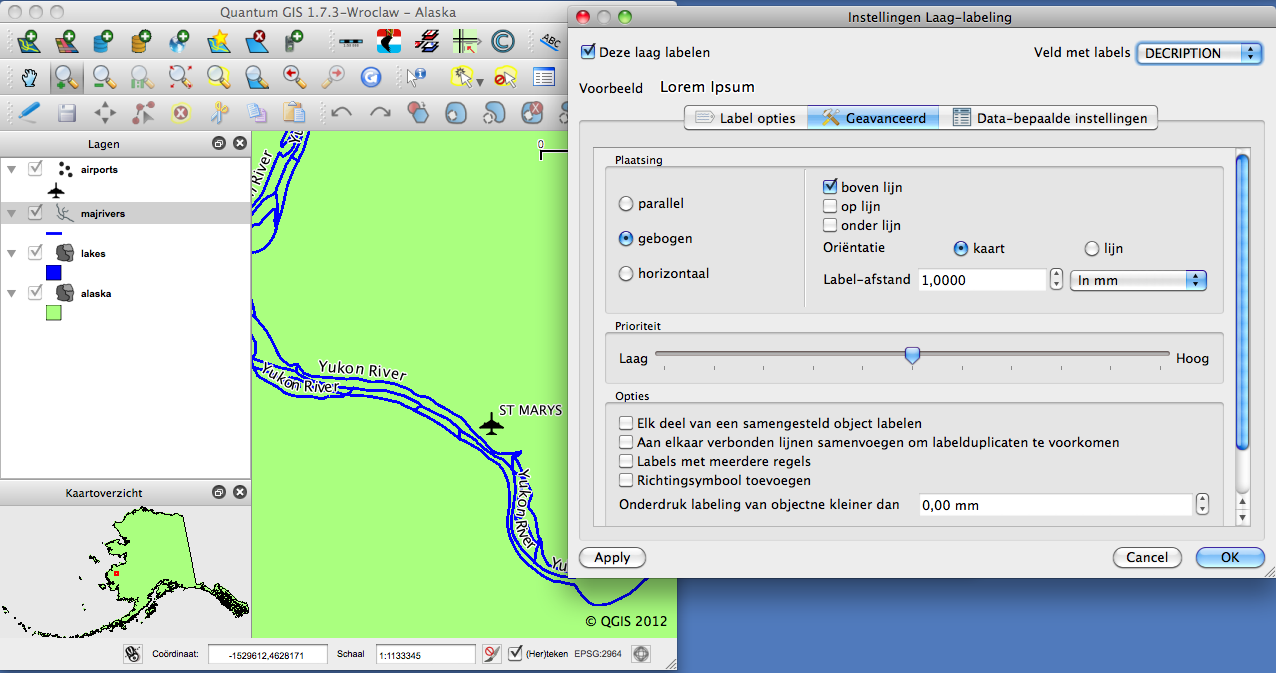
\includegraphics[clip=true, width=10cm]{label_line}
   \caption{Smart labeling of vector line layers \nixcaption}\label{fig:linelabel}
\end{figure}

\minisec{Labeling polygon layers}

First step is to activate the \checkbox{Label this layer} checkbox and select an attribute
column to use for labeling. After that you can define the label placement, distance and text
style, labeling priority, scale-based visibility, if every part of multipart feature is to be
labeled and if features act as obstacles for labels or not (see Figure \ref{fig:arealabel}).

\begin{figure}[ht]
\centering
   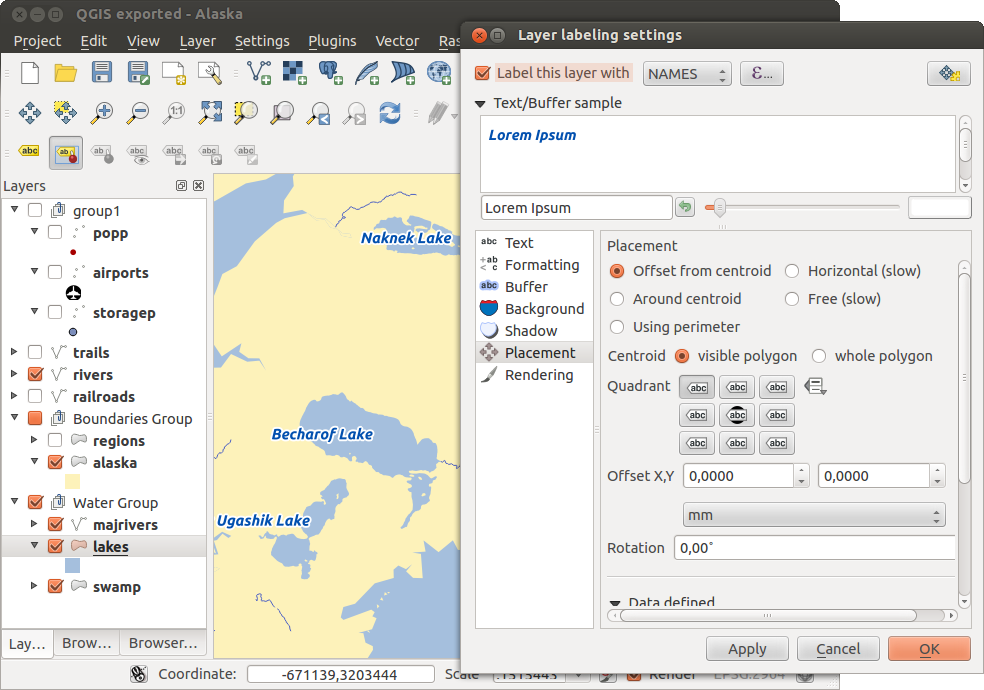
\includegraphics[clip=true, width=10cm]{label_area}
   \caption{Smart labeling of vector polygon layers \nixcaption}\label{fig:arealabel}
\end{figure}

\minisec{Change engine settings}

Additionally you can click the \button{Engine settings} button and select the search method,
used to find the best label placement. Available is Chain, Popmusic Tabu, Popmusic Chain,
Popmusic Tabu Chain and FALP.

\begin{figure}[ht]
\centering
   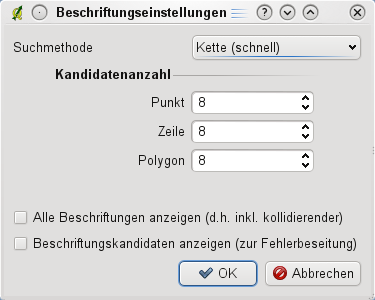
\includegraphics[clip=true, width=5cm]{label_engine}
   \caption{Dialog to change label engine settings \nixcaption}\label{fig:labelengine}
\end{figure}

Furthermore the number of candidates can be defined for point, line and polygon features,
and you can define whether to show all labels (including colliding labels) and label
candidates for debugging.

\subsection{Attributes Tab}\index{Attributes}\label{label_attributes}

Within the \tab{Attributes} tab the attributes of the selected dataset can be
manipulated. The buttons \toolbtntwo{mActionNewAttribute}{New Column} and
\toolbtntwo{mActionDeleteAttribute}{Delete Column} can be
used, when the dataset is \toolbtntwo{mActionToggleEditing}{Editing mode}.
At the moment only columns from PostGIS layers can be removed and added. The
OGR library supports to add new columns, but not to remove them, if you have
a GDAL version >= 1.6 installed.

\minisec{edit widget}

\begin{figure}[ht]
   \centering
   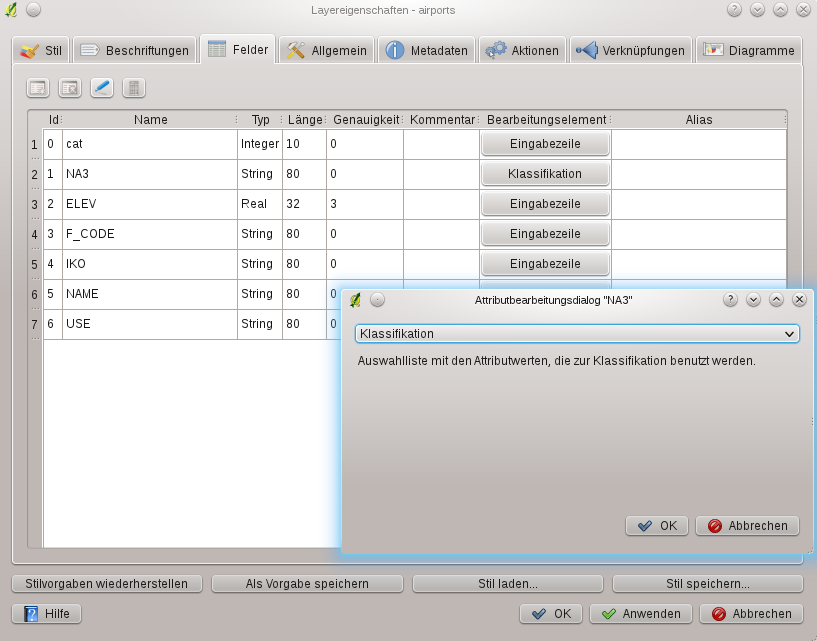
\includegraphics[clip=true, width=12cm]{editwidgetsdialog}
   \caption{Dialog to select an edit widget for an attribute column
\nixcaption}\label{fig:editwidget}
\end{figure}

Within the \tab{Attributes} tab you also find an \texttt{edit widget} column.
This column can be used to define values or a range of values that are
allowed
to be added to the specific attribute table column. If you click on the
\button{edit widget} button, a dialog opens, where you can define different
widgets. These widgets are:

\begin{itemize}[label=--]
\item Line edit: an edit field which allows to enter simple text (or restrict
to
numbers for numeric attributes).
\item Classification: Displays a combo box with the values used for
classification, if you have chosen 'unique value' as legend type in the
symbology tab of the properties dialog.
\item Range: Allows to set numeric values from a specific range. The edit
widget can be either a slider or a spin box.
\item Unique value: The user can select one of the values already used in the
attribute table. If editable is activated, a line edit is shown with
autocompletion support, otherwise a combo box is used.
\item File name: Simplifies the selection by adding a file chooser dialog.
\item Value map: a combo box with predefined items. The value is stored in
the attribute, the description is shown in the comboo box. You can define
values manually or load them from a layer or a CSV file.
\item Enumeration: Opens a combo box with values that can be used within the
columns type. This is currently only supported by the postgres provider.
\item Immutable: The immutable attribute column is read-only. The user is not
able to modify the content.
\item Hidden: A hidden attribute column is invisible. The user is not able to 
see its content. 
\item Checkbox: Displays a checkbox and you can define what attribute is added 
to the column when the checkbox is activated or not.
\item Text edit: This opens a text edit field that allows multiple lines to be 
used. 
\item Calendar: Opens a calendar widget to enter a date. Column type must be text.
\end{itemize}

\subsection{General Tab}\label{vectorgeneraltab}

The \tab{General} tab is essentially like that of the raster dialog. It
allows you to change the display name, set scale dependent rendering options,
create a spatial index of the vector file (only for OGR supported formats and
PostGIS) and view or change the projection of the specific vetor layer.

The \button{Query Builder} button allows you to create a subset of the
features in the layer - but this button currently only is available when you
open the attribute table and select the \button{...} button next to Advanced
search.

\subsection{Metadata Tab}\index{Metadata}

The \tab{Metadata} tab contains general information about the layer,
including specifics about the type and location, number of features, feature
type, and the editing capabilities. The \guiheading{Extents} section,
providing
layer extent information, and the \guiheading{Layer Spatial Reference System}
section, providing information about the CRS of the layer. This is a quick
way to get information about the layer, but is not yet editable.

\subsection{Actions Tab}\index{Actions}\label{label_actions}

\qg provides the ability to perform an action based on the attributes of a
feature. This can be used to perform any number of actions, for example,
running a program with arguments built from the attributes of a feature or
passing parameters to a web reporting tool.

Actions are useful when you frequently want to run an external application or
view a web page based on one or more values in your vector layer. An example
is performing a search based on an attribute value. This concept is used in
the following discussion.

\minisec{Defining Actions}\index{actions!defining}

Attribute actions are defined from the vector \dialog{Layer Properties} dialog. To
define an action, open the vector \dialog{Layer Properties} dialog and click on the
\tab{Actions} tab. Provide a descriptive name for the action. The action
itself must contain the name of the application that will be executed when the
action is invoked. You can add one or more attribute field values as arguments
to the application. When the action is invoked any set of characters that
start with a \% followed by the name of a field will be replaced by the value of
that field. The special characters \%\% \index{\%\%}will be replaced by the value
of the field that was selected from the identify results or attribute table (see
Using Actions below).  Double quote marks can be used to group text into a
single argument to the program, script or command. Double quotes will be
ignored if preceded by a backslash.

If you have field names that are substrings of other field names (e.g., \usertext{col1}
and \usertext{col10}) you should
indicate so, by surrounding the field name (and the \% character) with square
brackets (e.g., \usertext{[\%col10]}). This will prevent the \usertext{\%col10} field
name being mistaken for the \usertext{\%col1} field name with a \usertext{0}
on the end. The brackets will be removed by \qg when it substitutes in the
value of the field. If you want the substituted field to be surrounded by square
brackets, use a second set like this: \usertext{[[\%col10]]}.

The \dialog{Identify Results} dialog box includes a {\em (Derived)} item that
contains information relevant to the layer type. The
values in this item can be accessed in a similar way to the other fields
by using preceeding the derived field name by \usertext{(Derived).}. For
example, a point layer has an \usertext{X} and \usertext{Y} field and the
value of these can be used in the action with \usertext{\%(Derived).X} and
\usertext{\%(Derived).Y}. The derived attributes are only available from the
\dialog{Identify Results} dialog box, not the \dialog{Attribute Table} dialog box.

Two example actions are shown below:\index{actions!examples}

\begin{itemize}[label=--]
  \item \usertext{konqueror http://www.google.com/search?q=\%nam}
  \item \usertext{konqueror http://www.google.com/search?q=\%\%}
\end{itemize}

In the first example, the web browser konqueror is invoked and passed a URL to
open. The URL performs a Google search on the value of the \usertext{nam} field
from our vector layer. Note that the application or script called by the
action must be in the path or you must provided the full path. To be sure, we could
rewrite the first example as: \usertext{/opt/kde3/bin/konqueror
http://www.google.com/search?q=\%nam}. This will ensure that the konqueror
application will be executed when the action is invoked.

The second example uses the \%\% notation which does not rely on a particular
field for its value. When the action is invoked, the \%\% will be replaced by
the value of the selected field in the identify results or attribute table.

\minisec{Using Actions}\index{actions!using}\label{label_usingactions}

Actions can be invoked from either the \dialog{Identify Results} dialog or an
\dialog{Attribute Table} dialog (recall that these dialogs can be opened by
clicking \toolbtntwo{mActionIdentify}{Identify Features} or
\toolbtntwo{mActionOpenTable}{Open Attribute Table}). To invoke an action,
right click on the record and choose the action from the popup menu. Actions
are listed in the popup menu by the name you assigned when defining the
actions. Click on the action you wish to invoke.

If you are invoking an action that uses the \%\% notation, right-click on the
field value in the \dialog{Identify Results} dialog or the
\dialog{Attribute Table} dialog that you wish to pass to the application or script.

Here is another example that pulls data out of a vector layer and inserts them
into a file using bash and the \usertext{echo} command (so it will only work
\nix or perhaps \osx). The layer in question has fields for a species name
\usertext{taxon\_name}, latitude \usertext{lat} and longitude
\usertext{long}. I would like to be able to
make a spatial selection of a localities and export these field values to a
text file for the selected record (shown in yellow in the \qg map area). Here is
the action to achieve this:

\begin{verbatim}
  bash -c "echo \"%taxon_name %lat %long\" >> /tmp/species_localities.txt"
\end{verbatim}

After selecting a few localities and running the action on each one, opening
the output file will show something like this:

\begin{verbatim}
  Acacia mearnsii -34.0800000000 150.0800000000
  Acacia mearnsii -34.9000000000 150.1200000000
  Acacia mearnsii -35.2200000000 149.9300000000
  Acacia mearnsii -32.2700000000 150.4100000000
\end{verbatim}

As an exercise we create an action that does a Google search on the
\filename{lakes} layer. First we need to determine the URL needed to perform a search on a
keyword. This is easily done by just going to Google and doing a simple
search, then grabbing the URL from the address bar in your browser. From this
little effort we see that the format is: \url{http://google.com/search?q=qgis},
where \usertext{\qg} is the search term. Armed with this information, we can
proceed:

\begin{enumerate}
\item Make sure the \filename{lakes} layer is loaded.
\item Open the \dialog{Layer Properties} dialog by double-clicking on the layer in the
  legend or right-click and choose \dropmenuopt{Properties} from the popup menu.
\item Click on the \tab{Actions} tab.
\item Enter a name for the action, for example \usertext{Google Search}.
\item For the action, we need to provide the name of the external program to
  run. In this case, we can use Firefox. If the program is not in
  your path, you need to provide the full path.
\item Following the name of the external application, add the URL used for
  doing a Google search, up to but not included the search term:
  \url{http://google.com/search?q=}
\item The text in the \guilabel{Action} field should now look like this:\\
  \usertext{firefox \url{http://google.com/search?q=}}
\item Click on the drop-down box containing the field names for the
  \usertext{lakes} layer. It's located just to the left of the
  \button{Insert Field} button.
\item From the drop-down box, select \selectstring{Field containing label}{NAMES} and click \button{Insert Field}.
\item Your action text now looks like this:\\ \usertext{firefox
  \url{http://google.com/search?q=\%NAMES}}
\item Fo finalize the action click the \button{Insert action} button.
\end{enumerate}

This completes the action and it is ready to use. The final text of the action
should look like this:

\usertext{firefox \url{http://google.com/search?q=\%NAMES}}

We can now use the action. Close the \dialog{Layer Properties} dialog and zoom in to an area
of interest. Make sure the \filename{lakes} layer is active and identify a
lake. In the result box you'll now see that our action is visible:

\begin{figure}[ht]
   \centering
   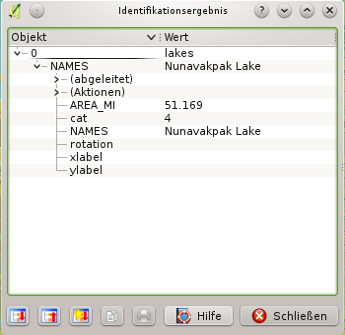
\includegraphics[clip=true, width=7cm]{action_identifyaction}
   \caption{Select feature and choose action \nixcaption}\label{fig:identify_action}
\end{figure}

When we click on the action, it brings up Firefox and navigates to the URL
\url{http://www.google.com/search?q=Tustumena}. It is also possible to add further
attribute fields to the action. Therefore you can add a ``+'' to the end of the action
text, select another field and click on \button{Insert Field}. In this example there
is just no other field available that would make sense to search for.

You can define multiple actions for a layer and each will show up in the
\dialog{Identify Results} dialog.
%% FIXME No longer valid??
%%You can also invoke actions from the attribute table
%%by selecting a row and right-clicking, then choosing the action from the popup
%%menu.

You can think of all kinds of uses for actions. For example, if you have a point layer
containing locations of images or photos along with a file name, you could
create an action to launch a viewer to display the image. You could also use
actions to launch web-based reports for an attribute field or combination of
fields, specifying them in the same way we did in our Google search example.

\subsection{Diagram Tab}\label{sec:diagram}
\index{vector layers!diagram}

The \tab{Diagram} tab allows you to add a grahic overlay to a vector layer.
To activate this feature, open the Plugin Manager and select the 'Diagram Overlay'
plugin. After this, there is a new tab in the vector \dialog{Layer
Properties} dialog where the settings for diagrams may be entered (see
figure~\ref{fig:diagramtab}).

\begin{figure}[ht]
   \centering
   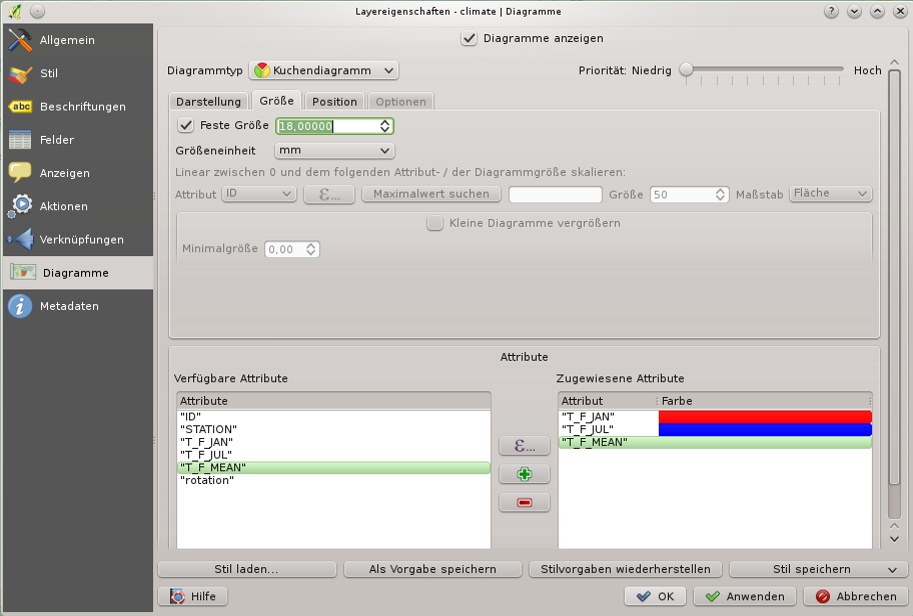
\includegraphics[clip=true, width=13cm]{diagram_tab}
   \caption{Vector properties dialog with diagram tab \nixcaption}\label{fig:diagramtab}
\end{figure}

The current implementation of diagrams provides support for piecharts, barcharts,
proportional SVG symbols, and for linear scaling of the diagram size according
to a classification attribute. We will demonstrate an example and overlay the
alaska boundary layer a barchart diagram showing some temperature data from
a climate vector layer. Both vector layers are part of the \qg sample dataset (see
Section~\ref{label_sampledata}.

\begin{enumerate}
\item First click on the \toolbtntwo{mActionAddOgrLayer}{Load Vector} icon,
browse to the \qg sample dataset folder and load the two vector shape layers
\filename{alaska.shp} and \filename{climate.shp}.
\item Double click the \filename{climate} layer in the map legend to open the
\dialog{Layer Properties} dialog.
\item Click on the \tab{Diagram Overlay} and select \button{Bar chart} as
Diagram type.
\item In the diagram we want to display the values of the three columns
\filename{T\_F\_JAN, T\_F\_JUL} and \filename{T\_F\_MEAN}. First select
\filename{T\_F\_JAN} as Attributes and click \button{Add attribute}, then
\filename{T\_F\_JUL} and finally \filename{T\_F\_MEAN}.
\item For linear scaling of the diagram size we define \filename{T\_F\_JUL}
as classification attribute.
\item Now click on \button{Find maximum value}, choose a size value and unit
and click \button{Apply} to display the diagram in the \qg main window.
\item You can now adapt the chart size, or change the attribute colors double
clicking on the color values in the attribute field.
Figure~\ref{fig:climatediagram} gives an impression.
\item Finally click \button{Ok}.
\end{enumerate}

\begin{figure}[ht]
   \centering
   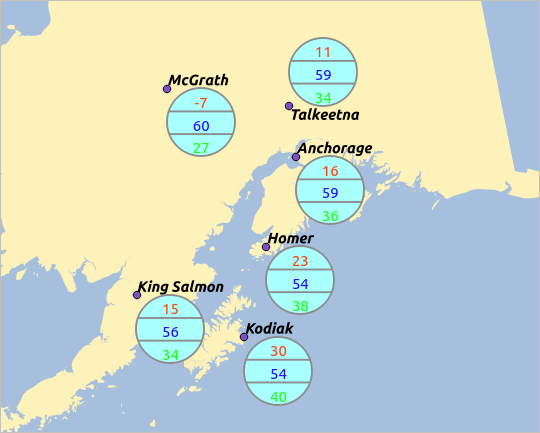
\includegraphics[clip=true, width=13cm]{climate_diagram}
   \caption{Diagram from temperature data overlayed on a map \nixcaption}\label{fig:climatediagram}
\end{figure}

\section{Editing}\index{editing}

\qg supports various capabilities for editing OGR, PostGIS and Spatialite
vector layers. \textbf{Note} - the procedure for editing GRASS layers is
different - see Section \ref{grass_digitising} for details.

\begin{Tip}\caption{\textsc{Concurrent Edits}}
This version of \qg does not track if somebody else is editing a
feature at the same time as you. The last person to save their edits wins.
\end{Tip}

\subsection{Setting the Snapping Tolerance and Search Radius}\label{snapping_tolerance}

Before we can edit vertices, we must set the snapping
tolerance and search radius to a value that allows us an optimal editing of
the vector layer geometries.

\minisec{Snapping tolerance}

Snapping tolerance is the distance \qg uses to \usertext{search} for the
closest vertex and/or segment you are trying to
connect when you set a new vertex or move an existing vertex. If you aren't
within the snap tolerance, \qg will leave the vertex where you release the
mouse button, instead of snapping it to an existing vertex and/or segment.
The snapping tolerance setting affects all tools which work with tolerance.

\begin{enumerate}
\item A general, project wide snapping tolerance can be defined choosing
\mainmenuopt{Settings} \arrow \dropmenuopttwo{mActionOptions}{Options}.
(On Mac: go to  \mainmenuopt{\qg} \arrow Preferences, on Linux: \mainmenuopt{Edit} \arrow \dropmenuopttwo{mActionOptions}{Options}.)
In the \tab{Digitizing} tab you can select between to vertex, to segment or
to vertex and segment as default snap mode. You can also define a default
snapping tolerance and a search radius for vertex edits. The tolerance an be
set either in map units or in pixels. The advantage of choosing pixels, is
that the snapping tolerance doesn't have to be changed after zoom operations.
In our small digitizing project (working with the Alaska dataset), we define
the snapping units in feet. Your results may vary, but something on the order
of 300ft should be fine at a scale of 1:10 000 should be a reasonable
setting.
\item A layer based snapping tolerance can be defined by choosing
\mainmenuopt{Settings} (or \mainmenuopt{File}) \arrow \dropmenuopttwo{mActionOptions}{Project
Properties\dots}. In the \tab{General} tab, section \classname{Digitize} you
can click on \button{Snapping options\dots} to enable and adjust snapping
mode and tolerance on a layer basis (see Figure~\ref{fig:snappingoptions}).
\end{enumerate}
Note that this layer based snapping overrides the global snapping option set in the Digitizing tab. So if you need to edit one layer, and snap its vertices to another layer, then enable snapping only on the \usertext{snap to} layer, then decrease the global snapping tolerance to a smaller value.  Furthermore, snapping will never occur to a layer which is not checked in the snapping options dialog, regardless of the global snapping tolerance. So be sure to mark the checkbox for those layers that you need to snap to.

\begin{figure}[ht]
   \centering
   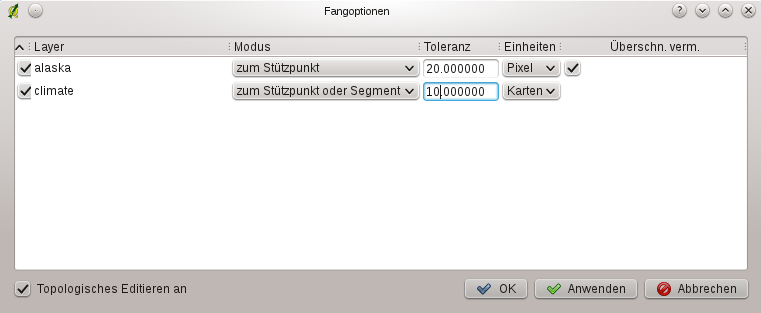
\includegraphics[clip=true, width=12cm]{editProjectSnapping}
   \caption{Edit snapping options on a layer basis \nixcaption}\label{fig:snappingoptions}
\end{figure}

\minisec{Search radius}

Search radius is the distance \qg uses to \usertext{search} for the closest
vertex you are trying to move when you click on the
map. If you aren't within the search radius, \qg won't find and select
any vertex for editing and it will pop up an annoying warning to that effect.
Snap tolerance and search radius are set in map units or pixels, so you may find you
need to experiment to get them set right. If you specify too big of a
tolerance, \qg may snap to the wrong vertex, especially if you are dealing
with a large number of vertices in close proximity. Set search radius too
small and it won't find anything to move.

The search radius for vertex edits in layer units can be defined in the
\tab{Digitizing} tab under \mainmenuopt{Settings} \arrow
\dropmenuopttwo{mActionOptions}{Options}. The same place where you define the
general, project wide snapping tolerance.

\subsection{Zooming and Panning}

Before editing a layer, you should zoom in to your area of interest. This
avoids waiting while all the vertex markers are rendered across the entire
layer.

Apart from using the \toolbtntwo{mActionPan}{pan} and
\toolbtntwo{mActionZoomIn}{zoom-in}/\toolbtntwo{mActionZoomOut}{zoom-out}
icons on the toolbar with the mouse, navigating can also be done with the
mouse wheel, spacebar and the arrow keys.

\minisec{Zooming and panning with the mouse wheel}

While digitizing you can press the mouse wheel to pan inside of the main
window and you can roll the mouse wheel to zoom in and out on the map. For
zooming place the mouse cursor inside the map area and roll it forward (away
from you)
to zoom in and backwards (towards you) to zoom out. The mouse cursor position
will
be the center of the zoomed area of interest. You can customize the behavior
of the mouse wheel zoom using the \tab{Map tools} tab under the
\mainmenuopt{Settings} \arrow \dropmenuopt{Options} menu.

\minisec{Panning with the arrow keys}

Panning the Map during digitizing is possible with the arrow keys. Place
the mouse cursor inside the map area and click on the right arrow key to
pan east, left arrow key to pan west, up arrow key to pan north and down
arrow key to pan south.

You can also use the spacebar to temporarily cause mouse movements to pan
then map. The PgUp and PgDown keys on your keyboard will cause the map
display to zoom in or out without interrupting your digitising session.

\subsubsection{Topological editing}

Besides layer based snapping options the \tab{General} tab in menu
\mainmenuopt{Settings} \arrow \dropmenuopttwo{mActionOptions}{Project Properties\dots}
also provides some topological functionalities.
In the Digitizing option group you can \checkbox{Enable topological editing} and/or activate
\checkbox{Avoid intersections of new polygons}.

\minisec{Enable topological editing}

The option \checkbox{Enable topological editing} is for editing and maintaining
common boundaries in polygon mosaics. \qg "detects" a shared boundary in
a polygon mosaic and you only have to move the vertex once and \qg will take
care about updating the other boundary.

\minisec{Avoid intersections of new polygons}

The second topological option called \checkbox{Avoid intersections of new polygons}
avoids overlaps in polygon mosaics. It is for quicker digitizing of adjacent polygons.
If you already have one polygon, it is possible with this option to digitise the second
one such that both intersect and \qg then cuts the second polygon to the common boundary.
The advantage is that users don't have to digitize all vertices of the common boundary.

\subsection{Digitizing an existing layer}
\index{vector layers!digitizing}
\index{digitizing!an existing layer}
\label{sec:edit_existing_layer}

By default, \qg loads layers read-only: This is a safeguard
to avoid accidentally editing a layer if there is a slip of the mouse.
However, you can choose to edit any layer as long as the data provider
supports it, and the underlying data source is writable (i.e. its files are
not read-only). Layer editing is most versatile when used on
PostgreSQL/PostGIS data sources.

In general, editing vector layers is divided into a digitizing and an advanced
digitizing toolbar, described in Section \ref{sec:advanced_edit}. You can
select and unselect both under \mainmenuopt{Settings} \arrow \dropmenuopt{Toolbars}.
Using the basic digitizing tools you can perform the following functions:

\begin{table}[ht]\index{vector layers!basic editing tools}
\centering
\begin{tabular}{|l|p{5.5cm}|l|p{5.5cm}|}
\hline \textbf{Icon} & \textbf{Purpose} & \textbf{Icon} & \textbf{Purpose} \\
\hline 
\includegraphics[width=0.7cm]{mActionToggleEditing}
   & Toggle editing
   & 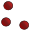
\includegraphics[width=0.7cm]{mActionCapturePoint}
   & Adding Features: Capture Point \\
\hline 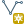
\includegraphics[width=0.7cm]{mActionCaptureLine}
   & Adding Features: Capture Line
   & 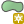
\includegraphics[width=0.7cm]{mActionCapturePolygon}
   & Adding Features: Capture Polygon \\
\hline 
\includegraphics[width=0.7cm]{mActionMoveFeature}
   & Move Feature
   & 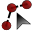
\includegraphics[width=0.7cm]{mActionNodeTool}
   & Node Tool \\
\hline 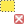
\includegraphics[width=0.7cm]{mActionDeleteSelected}
   & Delete Selected
   & 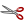
\includegraphics[width=0.7cm]{mActionEditCut}
   & Cut Features \\
\hline 
\includegraphics[width=0.7cm]{mActionEditCopy}
   & Copy Features
   & 
\includegraphics[width=0.7cm]{mActionEditPaste}
   & Paste Features \\
\hline 
\includegraphics[width=0.7cm]{mActionFileSave}
   & Save edits and continue
   &  &  \\
\hline
\end{tabular}
\caption{Vector layer basic editing toolbar}\label{tab:vector_editing}\medskip
\end{table}

All editing sessions start by choosing the
\dropmenuopttwo{mActionToggleEditing}{Toggle editing} option.
This can be found in the context menu after right clicking on the legend
entry for that layer.\index{Allow Editing}

Alternately, you can use the \index{Toggle Editing}
\toolbtntwo{mActionToggleEditing}{Toggle editing} button from the digitizing
toolbar to start or stop the editing mode.\index{editing!icons} Once the
layer is in edit mode, markers will appear at the vertices, and additional
tool buttons on the editing toolbar will become available.

\begin{Tip}\caption{\textsc{Save Regularly}}
Remember to toggle \toolbtntwo{mActionToggleEditing}{Toggle editing}
off regularly. This allows you to save your recent changes, and also confirms
that your data source can accept all your changes.
\end{Tip}

\minisec{Adding Features}
\index{vector layers!adding!feature}
\index{vector layers!move!feature}

You can use the \toolbtntwo{mActionCapturePoint}{Capture point},
\toolbtntwo{mActionCaptureLine}{Capture line} or
\toolbtntwo{mActionCapturePolygon}{Capture polygon} icons on the toolbar to
put the \qg cursor into digitizing mode.

For each feature, you first digitize the geometry, then enter its attributes.
To digitize the geometry, left-click on the map area to create the first
point of your new feature.

For lines and polygons, keep on left-clicking for each additional
point you wish to capture.  When you have finished adding points,
right-click anywhere on the map area to confirm you have finished entering
the geometry of that feature.

The attribute window will appear, allowing you to enter the information for
the new feature. Figure \ref{fig:vector_digitising} shows setting attributes
for a fictitious new river in Alaska. In the \tab{Digitising} tab under the
\mainmenuopt{Settings} \arrow \dropmenuopt{Options} menu, you can also activate the
\\
\checkbox{Suppress attributes pop-up windows after each created feature}.

\begin{figure}[ht]
   \centering
   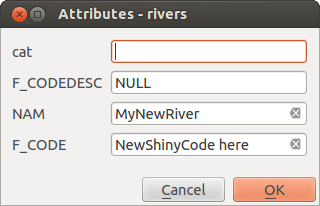
\includegraphics[clip=true, width=8cm]{editDigitizing}
   \caption{Enter Attribute Values Dialog after digitizing a new vector feature \nixcaption}\label{fig:vector_digitising}
 \end{figure}

With the \toolbtntwo{mActionMoveFeature}{Move Feature} icon on the toolbar
you can move existing features.

\begin{Tip}\caption{\textsc{Attribute Value Types}}
At least for shapefile editing the attribute types are validated during the
entry. Because of this, it is not possible to enter a number into the text-column in
the dialog \dialog{Enter Attribute Values} or vica versa. If you need to do so,
you should edit the attributes in a second step within the \dialog{Attribute
table} dialog.
\end{Tip}

\minisec{Node Tool}
\index{vector layers!node!tool}

For both PostgreSQL/PostGIS and shapefile-based layers, the
\toolbtntwo{mActionNodeTool}{Node Tool} provides manipulation capabilites
of feature vertices similar to CAD programs. It is possible to simply select
multiple vertices at once and to move, add or delete them alltogether. The node
tool also works with 'on the fly' projection turned on and supports
the topological editing feature. This tool is, unlike other tools in Quantum GIS,
persistent, so when some operation is done, selection stays active for this
feature and tool. If the node tool couldn't find any features, a warning will be
displayed.

Important is to set the property \mainmenuopt{Settings} \arrow
\dropmenuopttwo{mActionOptions}{Options} \arrow
\tab{Digitizing} \arrow \selectnumber{Search Radius}{10} to a number greater than
zero. Otherwise \qg will not be able to tell which vertex is being edited.

\begin{Tip}\caption{\textsc{Vertex Markers}}
The current version of \qg supports three kinds of vertex-markers -
Semi transparent circle, Cross and None. To change the marker style, choose
\dropmenuopttwo{mActionOptions}{Options} from the \mainmenuopt{Settings} menu
and click on the \tab{Digitizing} tab and select the appropriate entry.
\end{Tip}

\minisec{Basic operations}\index{vector layers!Node Tool}

Start by activating the \toolbtntwo{mActionNodeTool}{Node Tool} and selecting
some features by clicking on it. Red boxes appear at each vertex of this feature.
This is basic select of the feature. Functionalities are:

\begin{itemize}[label=--]
\item \textbf{Selecting vertex}: Selecting is easy just click on vertex and
color of this vertex will change to blue. When selecting more vertices
\keystroke{Shift} key can be used to select more vertices. Or also the
\keystroke{Ctrl} key can be used to invert selection of vertices (if selected then
it will be unselected and when not selected vertex will be selected). Also more
vertices can be selected at once when clicking somewhere outside feature and opening a rectangle where all vertices inside will be selected. Or just click on an edge and
both adjacent vertices should be selected.
\item \textbf{Adding vertex}: Adding vertex is simple, too. Just double click near
some edge and a new vertex will appear on the edge near to the cursor. Note that
vertex will appear on edge not on cursor position, there it has to be moved if
necessary.
\item \textbf{Deleting vertex}: After selecting vertices for deletion, click the
\keystroke{Delete} key and vertices will be deleted. Note that according to
standard Quantum GIS behavior, it will leave a necessary number of vertices for
the feature type you are working on. To delete a complete feature, another tool
has to be used.
\item \textbf{Moving vertex}: Select all vertices you want to move. All selected
vertices are moving in the same direction as the cursor. If snapping is enabled,
the whole selection can jump to the nearest vertex or line.
\end{itemize}

The \button{Release} button stores all changes and a new entry appears in the undo
dialog. Remember that all operations support topological editing when turned on. On
the fly projection is also supported.

\minisec{Cutting, Copying and Pasting Features}
\index{vector layers!cut!feature}
\index{vector layers!copy!feature}
\index{vector layers!paste!feature}
\index{editing!cutting features}
\index{editing!copying features}
\index{editing!pasting features}

Selected features can be cut, copied and pasted between layers in the
same \qg project, as long as destination layers are set to
\toolbtntwo{mActionToggleEditing}{Toggle editing} beforehand.

Features can also be pasted to external applications as text:  That is,
the features are represented in CSV format with the geometry data appearing
in the OGC Well-Known Text (WKT) format.

However in this version of \qg, text features from outside \qg cannot
be pasted to a layer within \qg. When would the copy and paste function
come in handy? Well, it turns out that you can edit more than one layer
at a time and copy/paste features between layers. Why would we want to do
this?  Say we need to do some work on a new layer but only need one or
two lakes, not the 5,000 on our \filename{big\_lakes} layer. We can create
a new layer and use copy/paste to plop the needed lakes into it.

As an example we are copying some lakes to a new layer:

\begin{enumerate}
\item Load the layer you want to copy from (source layer)
\item Load or create the layer you want to copy to (target layer)
\item Start editing for target layer
\item Make the source layer active by clicking on it in the legend
\item Use the \toolbtntwo{mActionSelect}{Select} tool to select the feature(s) on the source layer
\item Click on the \toolbtntwo{mActionEditCopy}{Copy Features} tool
\item Make the destination layer active by clicking on it in the legend
\item Click on the \toolbtntwo{mActionEditPaste}{Paste Features} tool
\item Stop editing and save the changes
\end{enumerate}

What happens if the source and target layers have
different schemas (field names and types are not the same)? \qg populates
what matches and ignores the rest. If you don't care about the attributes
being copied to the target layer, it doesn't matter how you design the
fields and data types. If you want to make sure everything - feature and its
attributes - gets copied, make sure the schemas match.

\begin{Tip}\caption{\textsc{Congruency of Pasted Features}}
If your source and destination layers use the
same projection, then the pasted features will have
geometry identical to the source layer.
However if the destination layer is a different projection
then \qg cannot guarantee the geometry is identical.
This is simply because there are small rounding-off errors
involved when converting between projections.
\end{Tip}

\minisec{Deleting Selected Features}
\index{vector layers!deleting!feature}

If we want to delete an entire polygon, we can do that by first selecting
the polygon using the regular \toolbtntwo{mActionSelect}{Select Features} tool. You can select
multiple features for deletion. Once you have the selection set, use the
\toolbtntwo{mActionDeleteSelected}{Delete Selected} tool to delete the features.

The \toolbtntwo{mActionEditCut}{Cut Features} tool on the digitizing toolbar can
also be used to delete features. This effectively deletes the feature but
also places it on a ``spatial clipboard". So we cut the feature to delete.
We could then use the \toolbtntwo{mActionEditPaste}{paste tool} to put it back, giving us a one-level undo
capability. Cut, copy, and paste work on the currently selected features,
meaning we can operate on more than one at a time.

\begin{Tip}\caption{\textsc{Feature Deletion Support}}
When editing ESRI shapefiles, the deletion
of features only works if \qg is linked to a GDAL version 1.3.2 or greater.
The OS X and Windows versions of \qg available from the download site are built
using GDAL 1.3.2 or higher.
\end{Tip}

\minisec{Saving Edited Layers}
\index{editing!saving changes}

When a layer is in editing mode, any changes remain in the memory of \qg.
Therefore they are not committed/saved immediately to the data source or disk.
If you want to save edits to the current layer but want to continue editing
without leaving the editing mode, you can click the
\toolbtntwo{mActionFileSave}{Save Edits} button. When you turn editing mode
off with the \toolbtntwo{mActionToggleEditing}{Toggle editing} (or quit
\qg for that matter), you are also asked if you want to save your changes
or discard them.

If the changes cannot be saved (e.g. disk full, or the attributes have
values that are out of range), the \qg in-memory state is preserved.  This
allows you to adjust your edits and try again.

\begin{Tip}\caption{\textsc{Data Integrity}}
It is always a good idea to back up your data source before you
start editing. While the authors of \qg have made every effort to preserve the
integrity of your data, we offer no warranty in this regard.
\end{Tip}

\subsection{Advanced digitizing}
\index{vector layers!advanced digitizing}
\index{advanced digitizing!an existing layer}
\label{sec:advanced_edit}

\begin{table}[h]\index{vector layers!advanced editing tools}
\centering
\small
\begin{tabular}{|l|p{6.9cm}|l|p{6.9cm}|}
\hline \textbf{Icon} & \textbf{Purpose} & \textbf{Icon} & \textbf{Purpose} \\
\hline \includegraphics[width=0.7cm]{mActionUndo}
   & Undo
   & \includegraphics[width=0.7cm]{mActionRedo}
   & Redo \\
\hline \includegraphics[width=0.7cm]{mActionSimplify}
   & Simplify Feature
   & \includegraphics[width=0.7cm]{mActionAddRing}
   & Add Ring \\
\hline \includegraphics[width=0.7cm]{mActionAddIsland}
   & Add Part
   & \includegraphics[width=0.7cm]{mActionDeleteRing}
   & Delete Ring \\
\hline \includegraphics[width=0.7cm]{mActionDeletePart}
   & Delete Part
   & \includegraphics[width=0.7cm]{mActionReshape}
   & Reshape Features \\
\hline \includegraphics[width=0.7cm]{mActionSplitFeatures}
   & Split Features
   & \includegraphics[width=0.7cm]{mActionMergeFeatures}
   & Merge Selected Features \\
\hline \includegraphics[width=0.7cm]{mActionRotatePointSymbols}
   & Rotate Point Symbols
   &
   & \\
\hline
\end{tabular}
\caption{Vector layer advanced editing toolbar}\label{tab:advanced_editing}
\end{table}

\minisec{Undo and Redo}
\index{vector layers!undo}
\index{vector layers!redo}

The \toolbtntwo{mActionUndo}{Undo} and \toolbtntwo{mActionRedo}{Redo} tools
allow the user to undo or redo the last or a certain step within the vector editing
operations. Basic view of Undo/Redo operations is a widget, where all operations
are shown (see Figure~\ref{fig:vector_redoundo}). This widget is not displayed by
default. Widget can be displayed by right clicking on toolbar and activating the
Undo/Redo check box. Undo/Redo is however active, even if the widget is not
displayed.

When Undo is hit, the state of all features and attributes are reverted to the
state before the reverted operation happened. Changes which are done elsewhere
(for example from some plugin), can show unspecific behavior for some operations
which appears in this box. The operations can be reverted or they stay the same.

An action can be triggered by clicking on Undo or Redo buttons or by clicking
directly on the item to which you want to return to. Another possibility to
trigger an undo operation is to click on the \button{undo/redo} buttons in
the advanced digitizing tool bar.

\begin{figure}[ht]
   \centering
   \includegraphics[clip=true, width=12cm]{redo_undo}
   \caption{Redo and Undo digitizing steps \nixcaption}\label{fig:vector_redoundo}
\end{figure}

\minisec{Simplify Feature}
\index{vector layers!simplify}

The \toolbtntwo{mActionSimplify}{Simplify Feature} tool allows to reduce the
number of vertices of a feature, as long as the geometry doesn't change. You
need to select a feature, it will be highlighted by a red rubber band and a
slider appears. Moving the slider, the red rubber band is changing its shape
to show how the feature is being simplified. Clicking \button{OK} the new,
simplified geometry will be stored. If a feature cannot be simplified (e.g.
MultiPolygons), a message shows up.

\minisec{Add Ring}
\index{vector layers!add!ring}

You can create ring polygons using the \toolbtntwo{mActionAddRing}{Add Ring}
icon in the toolbar. This means inside an existing area it is
possible to digitize further polygons, that will occur as a 'hole', so only
the area in between the boundaries of the outer and inner polygons remain as
a ring polygon.

\minisec{Add Part}
\index{vector layers!add!part}

You can \toolbtntwo{mActionAddIsland}{add part} polygons to a selected multipolygon.
The new part polygon has to be digitized outside the selected multipolygon.

\minisec{Delete Ring}
\index{vector layers!delete!ring}

The \toolbtntwo{mActionDeleteRing}{Delete Ring} tool allows to delete ring
polygons inside an existing area. This tool only works with polygon layers.
It doesn't change anything when it is used on the outer ring of the polygon.
This tool can be used on polygon and mutli-polygon features. Before
you select the vertices of a ring, adjust the vertex edit tolerance.

\minisec{Delete Part}
\index{vector layers!delete!part}

The \toolbtntwo{mActionDeletePart}{Delete Part} tool allows to delete parts
from multifeatures (e.g. to delete polygons from a multipolygon feature). It
won't delete the last part of the feature, this last part will stay untouched.
This tool works with all multi-part geometries point, line and polygon. Before
you select the vertices of a part, adjust the vertex edit tolerance.

\minisec{Reshape Features}
\index{vector layers!reshape!feature}

You can reshape line and polygon features using the
\toolbtntwo{mActionReshape}{Reshape Features} icon on the toolbar. It
replaces the line or polygon part from the first to the last intersection
with the original line. With polygons this can sometime lead to unintended
results. It is mainly useful to replace smaller parts of a polygon, not major
overhauls and the reshapeline is not allowed to cross several polygon rings
as this would generate an invalide polygon.

\textbf{Note}: The reshape tool may alter the starting position of a polygon
ring or a closed line. So the point that is represented 'twice' will not be
the same any more. This may not be a problem for most applications, but it is
something to consider.

\minisec{Split Features}
\index{vector layers!split!feature}

You can split features using the \toolbtntwo{mActionSplitFeatures}{Split
Features} icon on the toolbar. Just draw a line across the feature you
want to split.

\minisec{Merge selected features}
\index{vector layers!merge!features}

The \toolbtntwo{mActionMergeFeatures}{Merge Selected Features} tool allows to
merge features that have common boundaries and the same attributes.

\minisec{Rotate Point Symbols}
\index{vector layers!rotate!symbol}

The \toolbtntwo{mActionRotatePointSymbols}{Rotate Point Symbols} tool
allows to change the rotation of point symbols in the map canvas, if
you have defined a rotation column from the attribute table of the point
layer in the \tab{Symbology} tab of the \dialog{Layer Properties}.
Otherwise the tool is inactive.

\begin{figure}[ht]
   \centering
   \includegraphics[clip=true, width=6cm]{rotatepointsymbol}
   \caption{Rotate Point Symbols \nixcaption}\label{fig:rotatepoint}
\end{figure}

To change the rotation, select a point feature in the map canvas and rotate
it holding the left mouse button pressed. A red arrow with the rotation value
will be visualized (see Figure~\ref{fig:rotatepoint}). When you release the
left mouse button again, the value will be updated in the attribute table.

\textbf{Note}: If you hold the \keystroke{Ctrl} key pressed, the rotation will be done
in 15 degree steps.

\subsection{Creating a new Shapefile and Spatialite layer}\label{sec:create shape}\index{editing!creating a new shape layer}

\qg allows to create new Shapefile layers and new Spatialite layers.
Creation of a new GRASS layer is supported within the GRASS-plugin. Please refer
to section \ref{sec:creating_new_grass_vectors} for more information on
creating GRASS vector layers.

\minisec{Creating a new Shapefile layer}\label{sec:create shape}\index{editing!creating a new shapefile layer}

To create a new Shape layer for editing, choose \button{new} \arrow
\toolbtntwo{mActionNewVectorLayer}{New Shapefile Layer} from the
\mainmenuopt{Layer} menu. The \dialog{New Vector Layer} dialog will be
displayed as shown in Figure \ref{fig:newvectorlayer}. Choose the type of
layer (point, line or polygon).

\begin{figure}[ht]
   \centering
   \includegraphics[clip=true, width=8cm]{editNewVector}
   \caption{Creating a new Shapefile layer Dialog \nixcaption}\label{fig:newvectorlayer}
\end{figure}

Note that \qg does not yet support creation of 2.5D
features (i.e. features with X,Y,Z coordinates) or measure features. At this
time, only shapefiles can be created. In a future version of \qg, creation of
any OGR or PostgreSQL layer type will be supported.

To complete the creation of the new Shapefile layer, add the desired attributes by
clicking on the \button{Add} button and specifying a name and type for the
attribute. Only \selectstring{Type}{real}, \selectstring{Type}{integer}, and
\selectstring{Type}{string} attributes are supported. Additionally and
according to the attribute type you can also define the width and precision
of the new attribute column. Once you are happy with the attributes, click
\button{OK} and provide a name for the shapefile. \qg will automatically add
a \filename{.shp} extension to the name you specify. Once
the layer has been created, it will be added to the map and you can edit it in
the same way as described in Section \ref{sec:edit_existing_layer} above.

\minisec{Creating a new SpatiaLite layer}\label{sec:create spatialite}\index{editing!creating a new spatialite layer}

To create a new SpatiaLite layer for editing, choose \button{new} \arrow
\toolbtntwo{mActionNewVectorLayer}{New SpatiaLite Layer} from the
\mainmenuopt{Layer} menu. The \dialog{New SpatiaLite Layer} dialog will be
displayed as shown in Figure \ref{fig:newspatialitelayer}.

\begin{figure}[ht]
   \centering
   \includegraphics[clip=true, width=8cm]{editNewSpatialite}
   \caption{Creating a New Spatialite layer Dialog \nixcaption}\label{fig:newspatialitelayer}
\end{figure}

First step is to select an existing Spatialite database or to create a new
Spatialite database. This can be done with the browse \button{...} button
to the right of the database field. Then add a name for the new layer and
define the layer type and the EPSG SRID. If desired you can select to
\checkbox{create an autoincrementing primary key}.

To define an attribute table for the new Spatialite layer, add the names
of the attribute columns you want to create with the according column type
and click on the \button{Add to attribute list} button. Once you are happy
with the attributes, click \button{OK}. \qg will automatically add the new
layer to the legend and you can edit it in the same way as described in
Section \ref{sec:edit_existing_layer} above.

The spatialite creation dialog allows to create multiple layers without
closing the dialog when you click \button{Apply}.

\subsection{Working with the Attribute Table}
\label{sec:attribute table}
\index{editing!working with the attribute table}

The attribute table displays features of a selected layer. Each row in the table
represents one map feature with its attributes shown in several columns. The
features in the table can be searched, selected, moved or even edited.

To open the attribute table for a vector layer, make the layer active by clicking
on it in the map legend area. Then use \mainmenuopt{Layer} from the main menu
and and choose \dropmenuopttwo{mActionOpenTable}{Open Attribute Table}
from the menu. It is also possible to rightlick on the layer and
choose \dropmenuopttwo{mActionOpenTable}{Open Attribute Table} from the
dropdown menu. This will open a new window which displays the attributes for
every feature in the layer (figure \ref{fig:attributetable}). The number of features
are shown in the attribute table title.

\begin{figure}[ht]
   \centering
   \includegraphics[clip=true, width=12cm]{vectorAttributeTable}
   \caption{Attribute Table for Alaska layer \nixcaption}\label{fig:attributetable}
\end{figure}

\minisec{Selecting features in an attribute table}

\textbf{A selected row} in the attribute table represents all attributes of a
selected feature in the layer. The attribute table reflects any changes
in the layer selection in the main window and vice versa. A changed selection
in the attribute table also causes a change in the selected feature set in the
main window and different layer feature selection means different rows are to be
selected.

Rows can be selected by clicking on the row number on the left side of the
row. Selecting a row doesn't change the current cursor position. \textbf{Multiple
rows} can be marked by holding the \keystroke{Ctrl} key. A \textbf{continuous
selection} can be made by holding the \keystroke{Shift} key and clicking on several
row headers on the left side of the rows. All rows between the current cursor
position and the clicked row are selected.

Each column can be sorted by clicking on its column header. A small arrow
indicates the sort order (downward pointing means descending values from the top
row down, upward pointing means ascending values from the top rown down).

For a \textbf{simple search by attributes} on only one column the \button{Look for}
field can be used. Select the field (column) from which the search should be
performed from the dropdown menu and hit the \button{Search} button. The number of
matching rows will appear in the status bar. For more complex searches use
the Advanced search \button{...}, which will lauch the Search Query Builder
described in Section \ref{sec:select_by_query}.

To show selected records only, use the checkbox \checkbox{Show selected records only}. To search selected records only, use the checkbox \checkbox{Search selected records only}. The other buttons at the bottom left of the attribute table window provide following functionality:

\begin{itemize}[label=--]
\item \toolbtntwo{mActionOpenTable}{Remove selection}
\item \toolbtntwo{mActionSelectedToTop}{Move selected to top}
\item \toolbtntwo{mActionInvertSelection}{Invert selection}
\item \toolbtntwo{mActionCopySelected}{Copy selected rows to clipboard} also with \keystroke{Ctrl-C}
\item \toolbtntwo{mActionZoomToSelected}{Zoom map to selected rows} also with \keystroke{Ctrl-J}
\item \toolbtntwo{mActionToggleEditing}{toggle editing mode} to edit single values
of attribute table and to enable functionalities described below.
\item \toolbtntwo{mActionDeleteSelected}{Delete Selected Features}
\item \toolbtntwo{mActionNewAttribute}{New Column} for PostGIS layers and for OGR layers with GDAL version >= 1.6.
\item \toolbtntwo{mActionDeleteAttribute}{Delete Column} only for PostGIS layers yet.
\item \toolbtntwo{mActionCalculateField}{Open field calcultor}
\end{itemize}

\minisec{Save selected features as new layer}
\index{editing!save selection as new layer}

The selected features can be saved as any OGR supported vector format and also
transformed into another Coordinate Reference System (CRS). Just open the right mouse
menu of the layer and click on \dropmenuopt{Save selection as} to define the
name of the output file, its format and CRS (see Section \ref{label_legend}). It is 
also possible to specify OGR creation options within the dialog.

\begin{Tip}\caption{\textsc{Manipulating Attribute data}}
Currently only PostGIS layers are supported for adding or dropping
attribute columns within this dialog. In future versions of \qg, other
datasources will be supported, because this feature was recently implemented
in GDAL/OGR > 1.6.0
\end{Tip}

\minisec{Working with non spatial attribute tables}
\index{editing!working with non spatial tables}

QGIS allows also to load non spatial tables. This includes currently tables supported 
by OGR, delimited text and the PostgreSQL provider. The tables can be used for field 
lookups or just generally browsed and edited using the table view. When you load the 
table you will see it in the legend field. It can be opened e.g. with the 
\dropmenuopttwo{mActionOpenTable}{Open Attribute Table} tool and is then editable 
like any other layer attribute table. 

As an example you can use columns of the non spatial table to define attribute values or 
a range of values that are allowed to be added to a specific vector layer during digitizing. 
Have a closer look at the edit widget in section~\ref{label_attributes} to find out more.

\section{Query Builder}\label{sec:query_builder}
\index{Query Builder}

The \button{Advanced search\dots} button opens the Query Builder and allows you to
define a subset of a table using a SQL-like WHERE clause, display the result in theh
main window and save it as a Shapefile. For example, if you have a
\filename{towns} layer
with a \usertext{population} field you could select only larger towns by entering
\usertext{population > 100000} in the SQL box of the query builder. Figure
\ref{fig:query_builder} shows an example of the query builder populated with
data from a PostGIS layer with attributes stored in PostgreSQL.
The Fields, Values and Operators sections help the user to construct the SQL-like

\begin{figure}[ht]
  \centering
    \includegraphics[clip=true, width=11.5cm]{queryBuilder}
    \caption{Query Builder \nixcaption}\label{fig:query_builder}
\end{figure}

The \textbf{Fields list} contains all attributes of the attribute table to be
searched. To add an attribute to the SQL where clause field, double click its
name in the Fields list. Generally you can use the various fields, values and
operators to construct the query or you can just type it into the SQL box.

The \textbf{Values list} lists the values of an attribute. To list all possible
values of an attribute, select the attribute in the Fields list and click the
\button{All} button\index{Query Builder!getting all values}. To list all values
of an attribute that are present in the sample table, select the attribute in
the Fields list and click the \button{Sample}
button\index{Query Builder!generating sample list}. To add a value to the SQL
where clause field, double click its name in the Values list.

The \textbf{Operators section} contains all usable operators. To add an operator
to the SQL where clause field, click the appropriate button. Relational operators
( = , > , \dots), string comparison operator ( LIKE ), logical operators ( AND , OR
, \dots) are available.

The \button{Clear} button clears the text in the SQL where clause text field. The
\button{Test} button shows a message box with the number of features satisfying
the current query, which is usable in the process of query construction. The
\button{OK} button closes the window and selects the features satisfying the
query. The \button{Cancel} button closes the window without changing the current
selection.

\begin{Tip}\caption{\textsc{Changing the Layer Definition}}\index{Query
Builder!changing layer definitions}
You can change the layer definition after it is loaded by altering
the SQL query used to define the layer. To do this, open the
vector \dialog{Layer Properties} dialog by double-clicking on the layer in the legend and click on the
\button{Query Builder} button on the \tab{General} tab. See Section
\ref{sec:vectorprops} for more information.
\end{Tip}

\minisec{Select by query}\label{sec:select_by_query}

With \qg it is possible also to select features using a similar query builder
interface to that used in \ref{sec:query_builder}. In the above section
the purpose of the query builder is to only show features meeting the
filter criteria as a 'virtual layer' / subset. The purpose of the select by
query function is to highlight all features that meet a particular criteria.
Select by query can be used with all vector data providers.

To do a `select by query' on a loaded layer, click on the
button \toolbtntwo{mActionOpenTable}{Open Table} to open the attribute table of the layer. Then
click the \button{Advanced...} button at the bottom. This starts the Query Builder
that allows to define a subset of a table and display it as described in Section
\ref{sec:query_builder}.

\minisec{Save selected features as new layer}
\index{Query Builder!save selection as new layer}

The selected features can be saved as any OGR supported vector format and also
transformed into another Coordinate Reference System (CRS). Just open the right mouse
menu of the layer and click on \dropmenuopt{Save selection as} to define the
name of the output file, its format and CRS (see Section \ref{label_legend}). It is 
also possible to specify OGR creation options within the dialog.

\section{Field Calculator}\label{sec:field_calculator}
\index{PostgreSQL!field calculator}
\index{PostGIS!field calculator}
\index{OGR!field calculator}
\index{field calculator!PostgreSQL}
\index{field calculator!PostGIS}
\index{field calculator!OGR}

The \toolbtntwo{mActionCalculateField}{Field Calculator} button in the
attribute table allows to perform calculations on basis of existing
attribute values or defined functions, e.g to calculate length or area
of geometry features. The results can be written to a new attribute column
or it can be used to update values in an already existing column. The creation
of new attribute fields is currently only possible in PostGIS and with OGR
formats, if GDAL version is >= 1.6.0.

You have to bring the vector layer in editing mode, before you can click on
the field calculator icon to open the dialog (see Figure
\ref{fig:field_calculator}). In the dialog you first have to select whether
you want to update an existing field, only update selected features or
create a new attribute field, where the results of the calculation will be added.

\begin{figure}[ht]
  \centering
    \includegraphics[clip=true, width=11.5cm]{fieldcalculator}
    \caption{Field Calculator \nixcaption}\label{fig:field_calculator}
\end{figure}

If you choose to add a new field, you need to enter a field name, a field type
(integer, real or string), the total field width, and the field precision.
For example, if you choose a field width of 10 and a field precision of 3 it
means you have 6 signs before the dot, then the dot and another 3 signs for the
precision.

The \textbf{Fields list} contains all attributes of the attribute table to be
searched. To add an attribute to the Field calculator expression field, double
click its name in the Fields list. Generally you can use the various fields,
values and operators to construct the calculation expression or you can just
type it into the box.

The \textbf{Values list} lists the values of an attribute field. To list all
possible values, select the attribute field in the Fields list and click the
\button{All} button\index{Field Calculator!getting all values}. To list all
values of an attribute field that are present in the sample table, select the
attribute in the Fields list and click the \button{Sample} button\index{Field
Calcultor!generating sample list}. The procedure is the same as for the Query
Builder. To add a value to the Field calculator expression box, double click its
name in the Values list.

The \textbf{Operators section} contains all usable operators. To add an operator
to the Field calculator expression box, click the appropriate button. Mathematical
calculations ( + , - , * \dots), trigonometric functions ( sin, cos, tan, \dots),
extract geometric information ( length and area ) are available, together with
concatenator (||) and row counter. Stay tuned for more operators to come!

A short example illustrates how the field calculator works. We want to calculate
the length of the 'railroads' layer from the \filename{\qg\_example\_dataset}:

\begin{enumerate}
\item Load the Shapefile \filename{railroads.shp} in \qg and open
the \dialog{Attribute Table} dialog.
\item Click on \toolbtntwo{mActionToggleEditing}{Toggle editing mode} and
open the \toolbtntwo{mActionCalculateField}{Field Calculator} dialog.
\item Unselect the \checkbox{Update existing field} checkbox to enable the
new field box.
\item Add 'length' as output field name, 'real' as output field type and define
output field width 10 and a precision of 3.
\item Now click on Operator 'length' to add it as \$length into the
field calculator expression box and click \button{Ok}.
\end{enumerate}
